\clearpage \documentclass[a4paper,12pt,notitlepage]{article}

\frenchspacing
\usepackage{a4}
\usepackage[pdftitle={Vypracovane otazky k bakalarskym statnicim}, pdfauthor={študenti MFF}, pdfdisplaydoctitle=true, colorlinks=false,unicode=true,pdfborder=0 0 0]{hyperref}
\usepackage{slovak}
\usepackage{ucs}
\usepackage[utf8x]{inputenc}

\title{Vypracovane otazky k bakalarskym statnicim}
\author{študenti MFF}

\usepackage{graphicx}
\usepackage{amsmath,amssymb,amsthm}
\usepackage{color}
\usepackage[left=3cm, right=3cm, top=3cm, bottom=3cm]{geometry} % nastavení dané velikosti okrajů


%Vacsina prostredi je dvojjazicne. V pripade, ze znenie napr pozorovania je pisane po slovensky, malo by byt po slovensky aj oznacenie.

\newenvironment{pozadavky}{\pagebreak[2]\noindent\textbf{Požadavky}\par\noindent\leftskip 10pt}{\par\bigskip}
\newenvironment{poziadavky}{\pagebreak[2]\noindent\textbf{Požiadavky}\par\noindent\leftskip 10pt}{\par\bigskip}

\newenvironment{definice}{\pagebreak[2]\noindent\textbf{Definice}\par\noindent\leftskip 10pt}{\par\bigskip}
\newenvironment{definiceN}[1]{\pagebreak[2]\noindent\textbf{Definice~}\emph{(#1)}\par\noindent\leftskip 10pt}{\par\bigskip}
\newenvironment{definicia}{\pagebreak[2]\noindent\textbf{Definícia}\par \noindent\leftskip 10pt}{\par\bigskip}
\newenvironment{definiciaN}[1]{\pagebreak[2]\noindent\textbf{Definícia~}\emph{(#1)}\par\noindent\leftskip 10pt}{\par\bigskip}

\newenvironment{pozorovani}{\pagebreak[2]\noindent\textbf{Pozorování}\par\noindent\leftskip 10pt}{\par\bigskip}
\newenvironment{pozorovanie}{\pagebreak[2]\noindent\textbf{Pozorovanie}\par\noindent\leftskip 10pt}{\par\bigskip}
\newenvironment{poznamka}{\pagebreak[2]\noindent\textbf{Poznámka}\par\noindent\leftskip 10pt}{\par\bigskip}
\newenvironment{poznamkaN}[1]{\pagebreak[2]\noindent\textbf{Poznámka~}\emph{(#1)}\par\noindent\leftskip 10pt}{\par\bigskip}
\newenvironment{lemma}{\pagebreak[2]\noindent\textbf{Lemma}\par\noindent\leftskip 10pt}{\par\bigskip}
\newenvironment{lemmaN}[1]{\pagebreak[2]\noindent\textbf{Lemma~}\emph{(#1)}\par\noindent\leftskip 10pt}{\par\bigskip}
\newenvironment{veta}{\pagebreak[2]\noindent\textbf{Věta}\par\noindent\leftskip 10pt}{\par\bigskip}
\newenvironment{vetaN}[1]{\pagebreak[2]\noindent\textbf{Věta~}\emph{(#1)}\par\noindent\leftskip 10pt}{\par\bigskip}
\newenvironment{vetaSK}{\pagebreak[2]\noindent\textbf{Veta}\par\noindent\leftskip 10pt}{\par\bigskip}
\newenvironment{vetaSKN}[1]{\pagebreak[2]\noindent\textbf{Veta~}\emph{(#1)}\par\noindent\leftskip 10pt}{\par\bigskip}

\newenvironment{dusledek}{\pagebreak[2]\noindent\textbf{Důsledek}\par\noindent\leftskip 10pt}{\par\bigskip}
\newenvironment{dosledok}{\pagebreak[2]\noindent\textbf{Dôsledok}\par\noindent\leftskip 10pt}{\par\bigskip}

\newenvironment{dokaz}{\pagebreak[2]\noindent\leftskip 10pt\textbf{Dôkaz}\par\noindent\leftskip 10pt}{\par\bigskip}
\newenvironment{dukaz}{\pagebreak[2]\noindent\leftskip 10pt\textbf{Důkaz}\par\noindent\leftskip 10pt}{\par\bigskip}

\newenvironment{priklad}{\pagebreak[2]\noindent\textbf{Příklad}\par\noindent\leftskip 10pt}{\par\bigskip}
\newenvironment{prikladSK}{\pagebreak[2]\noindent\textbf{Príklad}\par\noindent\leftskip 10pt}{\par\bigskip}
\newenvironment{priklady}{\pagebreak[2]\noindent\textbf{Příklady}\par\noindent\leftskip 10pt}{\par\bigskip}
\newenvironment{prikladySK}{\pagebreak[2]\noindent\textbf{Príklady}\par\noindent\leftskip 10pt}{\par\bigskip}

\newenvironment{algoritmusN}[1]{\pagebreak[2]\noindent\textbf{Algoritmus~}\emph{(#1)}\par\noindent\leftskip 10pt}{\par\bigskip}
%obecne prostredie, ktore ma vyuzitie pri specialnych odstavcoch ako (uloha, algoritmus...) aby nevzniklo dalsich x prostredi
\newenvironment{obecne}[1]{\pagebreak[2]\noindent\textbf{#1}\par\noindent\leftskip 10pt}{\par\bigskip}


\newenvironment{penumerate}{
\begin{enumerate}
  \setlength{\itemsep}{1pt}
  \setlength{\parskip}{0pt}
  \setlength{\parsep}{0pt}
  %\setlength{\topsep}{200pt}
  \setlength{\partopsep}{200pt}
}{\end{enumerate}}

\def\pismenka{\numberedlistdepth=2} %pouzit, ked clovek chce opismenkovany zoznam...

\newenvironment{pitemize}{
\begin{itemize}
  \setlength{\itemsep}{1pt}
  \setlength{\parskip}{0pt}
  \setlength{\parsep}{0pt}
}{\end{itemize}}

\definecolor{gris}{gray}{0.95}
\newcommand{\ramcek}[2]{\begin{center}\fcolorbox{white}{gris}{\parbox{#1}{#2}}\end{center}\par}
 \clearpage
\title{\LARGE Učební texty k státní bakalářské zkoušce \\ Obecná informatika \\ Architektury počítačů a sítí}
\begin{document}
\maketitle
\newpage
\setcounter{section}{4}
\section{Architektury počítačů a sítí}
\begin{pozadavky}
\begin{pitemize}
\item Architektury počítače.
\item Procesory, multiprocesory.
\item Vstupní a výstupní zařízení, ukládání a přenos dat.
\item Architektury OS.
\item Procesy, vlákna, plánování.
\item Synchronizační primitiva, vzájemné vyloučení.
\item Zablokování a zotavení z něj.
\item Organizace paměti, alokační algoritmy.
\item Principy virtuální paměti, stránkování.
\item Systémy souborů, adresářové struktury.
\item Bezpečnost, autentifikace, autorizace, přístupová práva.
\item ISO/OSI vrstevnatá architektura sítí.
\item TCP/IP.
\item Spojované a nespojované služby, spolehlivost, zabezpečení protokolů.
\end{pitemize}
\end{pozadavky}
\subsection{Architektury počítače}

\begin{definiceN}{Architektura počítača}
Architektura počítača popisuje \uv{všetko, čo by mal vedieť ten, ktorý programuje v assembleri / tvorí operačný systém}. Teda:
\begin{pitemize}
	\item z akých častí -- štruktúra počítača, usporadanie
	\item význam častí -- funkcia časti, ich vnútorná štruktúra
	\item ako spolu časti komunikujú -- riadenie komukácie
	\item ako sa jednotlivé časti ovládajú, aká je ich funkčnosť navonok
\end{pitemize}
\end{definiceN}

\begin{definiceN}{Víceúrovňová organizace počítače}
\begin{pitemize}
	\item Mikroprogramová úroveň (priamo technické vybavenie počítača)
	\item Strojový jazyk počítače (virtuálny stroj nad obvodovým riešením; vybavenie~-- popis architektúry a organizácie)
	\item Úroveň operačního systému (doplnenie predchádzajúcej úrovne o súbor makroinštrukcií a novú organizáciu pamäti)
	\item Úroveň assembleru (najnižšia úroveň ľudsky orientovaného jazyka)
	\item Úroveň vyšších programovacích jazyků (obecné alebo problémovo orientované; prvá nestrojovo orientovaná úroveň)
	\item Úroveň aplikačních programů
\end{pitemize}
\end{definiceN}


\begin{obecne}{Je teda potrebné definovať}
\begin{pitemize}
	\item Inštrukčný súbor (definícia prechodovej funkcie medzi stavmi počítača, formát inštrukcie, spôsob zápisu, možnosti adresovania operandov)
	\item Registrový model (rozlišovanie registrov procesoru: podľa voľby, pomocou určenia registru~-- explicitný/implicitný register; podľa funkcie registru~-- riadiaci~register/register~operandu)
	\item Definice specializovaných jednotek (jednotka na výpočet vo floatoch;\\fetch/decode/execute jednotky)
	\item Paralelismy (rozklad na úlohy, ktoré sa dajú spracovať súčasne~-- granularita (programy, podprogramy, inštrukcie...))
	\item Stupeň predikce (schopnosť pripraviť sa na očakávanú udalosť (načítanie inštrukcie, nastavenie prenosu dát)~-- explicitná predikcia, štatistika, heuristiky, adaptívna predikcia)

\bigskip
	\item Datové struktury a reprezentáciu dát (spôsob uloženia dát v počítači, mapovacie funkcie medzi reálnym svetom a vnútorným uložením, minimálna a maximálna veľkosť adresovateľné jednotky)
	\item Adresové konvencie (ako sa pristupuje k dátovým štruktúram~-- \emph{segment+offset} alebo \emph{lineárna adresácia}; veľkosť pamäti a jej šírika, \uv{povolené} miesta)

\bigskip
	\item Řízení (spolupráca procesoru a ostatných jednotiek, interakcia s okolím, prerušenia~-- vnútorne/vonkajšie)
	\item Vstupy a výstupy (metódy prenosu dát medzi procesorom a ostatnými jednotkami/počítačom a okolím; zahrňuje definície dátových štruktúr, identifikácia zdroja/cieľa, dátových ciest, protokoly, reakcie na chyby).
	\item Šíře datových cest
	\item Stupeň sdílení (na úrovni obvodov~-- zdieľanie obvodov procesoru a IO; na úrovni jednotiek~-- zdieľanie ALU viacerými procesormi)
\end{pitemize}
\end{obecne}

\subsubsection*{Základní dvě architektury počítačů}

\begin{obecne}{Von Neumannova}
  \begin{pitemize}
      \item Počítač se skládá z řídící jednotky, ALU, paměti a I/O jednotek
      \item Štruktúra počítača sa nemení typom úlohy (tj. počítač je programovaný obsahem paměti). %to tuetschek sorry neumim cist... ajs
      \item Program se nejprve zavede do paměti, z ní se postupně popořadě vybírají instrukce (a následující krok závisí na předchozím), pořadí lze změnit instrukcemi skoku. 
      \item Do jedné paměti, dělené na buňky stejné velikosti, se ukládají i zpracovávaná data. Data jsou reprezentovaná binárně. 
      \item V každém okamžiku je vykonávána jen jedna činnost. Je to architektura SISD (viz Flynnova taxonomie).
  \end{pitemize}

  Je pevně daná instrukční sada. Strojová instrukce obsahuje operační znak, který určuje druh operace, počet parametrů atd., a operandovú část~-- umístnění jednotlivých operandů. Vykonat jednu instrukci znamená:
  \begin{pitemize}
	  \item (fetch) načítať inštrukciu z pamäti do procesoru
	  \item (decode) zistiť o akú inštrukciu ide
	  \item (load) pripraviť zdrojové operandy
	  \item (execute) vykonať operáciu
	  \item (store) uloziť cieľové operandy
  \end{pitemize}

  Při vykonávání programu jsou potřebné různé registry~-- nejdůležitější jsou: PC (Program Counter, obsahuje adresu následující instrukce), IR (Instruction Register, adresa právě vykonávané instrukce), SP (Stack Pointer, ukazatel na vrchol zásobníku), MAR (memory access register~-- adresa do operační paměti), MBR (memory buffer register, dáta čítána/zapisována do paměti).

  Struktura jednoprocesorového počítače podle Von Neumanna:
  \begin{center}
    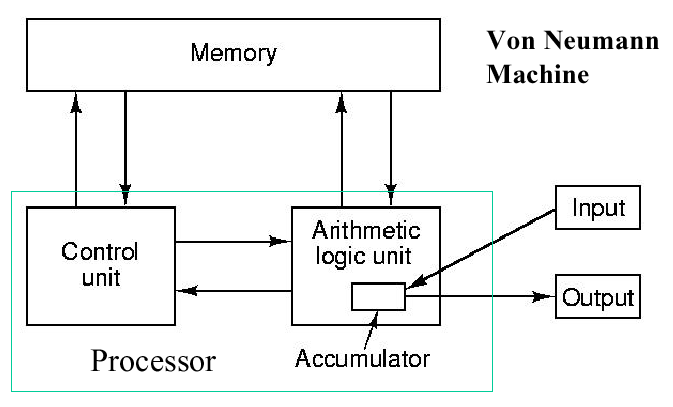
\includegraphics[width=8cm]{informatika/operacne_systemy_a_hw/obrazky/VonNeumann.png}
  \end{center}
\end{obecne}

\begin{obecne}{Harvardská}
Vytvořena až po Von Neumannově, liší se hlavně tím, že program se ukládá do jiné paměti než data (tzn. jsou 2 \uv{druhy paměti}~-- instrukcí a dat). Příklady jsou DSP procesory a mikrokontrolery (např. AVR od Atmelu, a PIC~-- mají paměť na program a data a RISC instrukční sadu; výhoda oddělených pamětí je, že můžou mít různou bitovou hloubku~-- 8 bitové data, ale 12-, 14- či 16- bitové instrukce (např. ARM musí občas použít více než jednou instrukci na zpracování obsahu plné velikosti)).

Oproti Von Neumannově nehrozí nebezpečí přepsání programu sebou samým, ale kvůli většímu počtu paměťových sběrnic je náročnější na výrobu. Paměť navíc nelze dělit podle potřeby (rozdělení je už dané).
\end{obecne}

\subsection{Procesory, multiprocesory}

\begin{definiceN}{Procesor} 
Procesor (CPU – central processing unit) je ústřední výkonnou jednotkou počítače, která čte z paměti instrukce a na jejich základě vykonává program.

Základnými súčasťami procesora sú:
\begin{pitemize}
	\item řadič nebo řídicí jednotka, která řídí tok programu, tj. načítání instrukcí, jejich dekódování, načítání operandů instrukcí z operační paměti a ukládání výsledků zpracování instrukcí
	\item sada registrů k uchování operandů a mezivýsledků.
	\item jedna nebo více aritmeticko-logických jednotek (ALU), které provádí s daty aritmetické a logické operace.
	\item některé procesory obsahují jednu nebo několik jednotek plovoucí čárky (FPU), které provádí operace v plovoucí řádové čárce.
\end{pitemize}
\end{definiceN}

\begin{poznamka}
Súčasné procesory navyše často obsahujú ďalšie rozsiahle funkčné bloky (cache, rôzne periférie)~-- ktoré z \uv{ortodoxného hladiska} nie sú priamo súčasťou \emph{jadra procesoru}. Niektoré procesory môžu obsahovať viac jadier (+logiku slúžiacu k ich vzájomnému prepojeniu). Ďalším trendom je SoC (System on Chip), kde sa na čipe procesora nachádzajú aj ďalšie subsystémy napr. na spracovanie zvuku, grafiky alebo pripojenie externých periférií (takéto riešenia sa využívajú väčšinou v PDA, domácej elektronike, mobiloch atď.).
\end{poznamka}

\begin{obecne}{Dělení podle instruční sady}
Podľa inštrukčnej sady je možné procesory rozdeliť na:
\begin{pitemize}
	\item \textbf{CISC} (Complex Instruction Set Computer): poskytuje rozsiahlu inštrukčnú sadu spolu s rôznymi variantami inštrukcií. Jedna inštrukcia napr. môže vykonať veľa low-level operácií (načítanie z pamäti, vykonať aritmetickú operáciu a výsledok uložiť). Takéto inštrukcie zjednodušovali zápis programov (inštrukcie boli bližšie vyšším programovacím jazykom) a zmenšovali veľkosť programu a počet prístupov do pamäti~-- čo bolo v 60tych rokoch dôležité. Avšak nie vždy je vykonanie jednej zložitej operácie rýchlejšie ako vykonanie viac menej zložitých miesto toho (napr. kvôli zložitému dekódovaniu a použitiu mikrokódu na volanie jednoduchých \uv{podinštrukcií}). Príkladmi CISC architektúr procesorov sú System/360, Motorola 68000 a Intel x86. V súčasnosti napr. x86 rozkladá zložité inštrukcie na \uv{micro-operations} ktoré môžu byť pipeline-ou spracované paralelne a vyšší výkon je tak dosahovaný na väčšom rozsahu inštrukcií. Vďaka tomu sú súčasné x86 procesory minimálne rovnako výkonné ako ozajstné RISC architektúry.
	\item \textbf{RISC} (Reduced Instruction Set Computer): design CPU ktorý uprednosňuje jednoduchšiu inštrukčnú sadu a menšiu zložitosť adresovacích modelov~-- vďaka čomu je možné dosiahnuť lacnejšiu implementáciu, väčšiu úroveň paralelizmu a účinnejšie kompilátory. Dôvodom vzniku bolo aj nevyužívanie celej CISC inštrukčnej sady a upredňostňovania len obmedzenej podmnožiny (designéri procesorov potom optimalizovali len tieto podmnožiny a tak sa zvyšné inštrukcie používali ešte menej...). Kvôli väčšiemu počtu inštrukcií však musia RISC procesory častejšie pristupovať k pamäti... Príkladmi RISC procesorov sú napr. SPARC a ARM. V architekturách typu \textbf{Post-RISC} jde o spojení RISCových vlastností s technikami zvýšení výkonu, jako je out-of-order vykonávání a paralelismus.
    \item \textbf{VLIW}: Very Long Instruction Word or VLIW refers to a CPU architecture designed to take advantage of instruction level parallelism (ILP). A processor that executes every instruction one after the other (i.e. a non-pipelined scalar architecture) may use processor resources inefficiently, potentially leading to poor performance. The performance can be improved by executing different sub-steps of sequential instructions simultaneously (this is pipelining), or even executing multiple instructions entirely simultaneously as in superscalar architectures. The VLIW approach, on the other hand, executes operation in parallel based on a fixed schedule determined when programs are compiled. Since determining the order of execution of operations (including which operations can execute simultaneously) is handled by the compiler, the processor does not need the scheduling hardware that the three techniques described above require. As a result, VLIW CPUs offer significant computational power with less hardware complexity (but greater compiler complexity) than is associated with most superscalar CPUs.
    \item \textbf{EPIC}: (Někdy označován za poddruh VLIW) Explicitly Parallel Instruction Computing (EPIC) is a computing paradigm that began to be researched in the 1990s. This paradigm is also called Independence architectures. It was used by Intel and HP in the development of Intel’s IA-64 architecture, and has been implemented in Intel’s Itanium and Itanium 2 line of server processors. The goal of EPIC was to increase the ability of microprocessors to execute software instructions in parallel, by using the compiler, rather than complex on-die circuitry, to identify and leverage opportunities for parallel execution. This would allow performance to be scaled more rapidly in future processor designs, without resorting to ever-higher clock frequencies, which have since become problematic due to associated power and cooling issues.
\end{pitemize}
\medskip
TODO: asi opravit, možná zpřesnit VLIW a EPIC a určitě přeložit

\medskip
Řekneme, že procesor má \emph{ortogonální instrukční sadu}, pokud žádná instrukce nepředpokládá implicitně použití některých registrů. To umožňuje jednodušší práci algoritmům přidělování registrů v překladačích. Příkladem neortogonální instrukční sady je i x86.
\end{obecne}

\begin{obecne}{Další dělení}
Ďalej je možné procesory rozdeliť podľa dĺžky operandov v bitoch (8, 16, 32, 64...), ktorý je procesor schopný spracovať v jednom kroku. V embedded zariadeniach sa najčastejšie používajú 4- a 8-bitové procesory. V PDA, mobiloch a videohrách 8 resp. 16 bitové. 32 a viac bitov využíajú napr. osobné počítače a laserové tlačiarne.

Dôležitou vlastnosťou je aj taktovacia frekvencia jadra, MIPS (millions of instructions per second) a jeho rýchlosť. V súčasnosti je ťažké dávať do súvislosti výkon procesorov s ich frekvenciou (resp. MIPS)~-- kým Pentium zvládne na výpočet vo floatoch, jednoduchý 8-bitový PIC na to potrebuje oveľa viac taktov. Ďalším \uv{problémom} je superskalarita procesorov, ktorá im umožňuje vykonať viacero nezávislých inštrukcií počas jedného taktu.
\end{obecne}

\begin{obecne}{Techniky pro zvýšení výkonu}
Zvyšovať výkon (procesorov) je možné viacerými spôsobmi. Najjednoduchším (a najpomalším) typom je Subskalárny CPU (načíta a spracúva len jednu inštrukciu naraz~-- preto musí celý procesor čakať kým vykonávanie inštrukcie skončí; je tak zdržovaný dlhšie trvajúcimi inštrukciami). 

\begin{center}
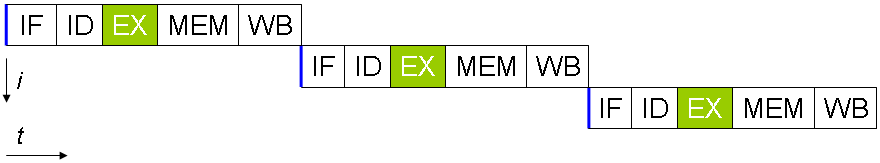
\includegraphics[width=8cm]{informatika/operacne_systemy_a_hw/obrazky/Nopipeline.png}
\end{center}

Pokusy o dosiahnutie skalárneho a lepšieho výkonu vyústili do designov ktoré sa správajú menej lineárne a viac paralelne. Čo sa týka paralelizmu v procesoroch, používajú sa dva druhy pojmov na ich klasifikáciu~-- \emph{Instruction level parallelism} (zvyšovanie rýchlosti vykonávania inštrukcií v procesore a teda zväčšovanie využitia prostriedkov na čipe) a \emph{Thread level parallelism} (zväčšovanie počtu vlákien, ktoré dokáže CPU vykonávať naraz).
\begin{pitemize}
  \item \textbf{pipeline}: 
  Zlepšenie je možné dosiahnúť pomocou \uv{instruction pipelining}-u, ktoré je použíté vo väčšine moderných procesorov. Umožňuje vykonanie viac ako jednej inštrukcie v jednom kroku vďaka rozloženiu spracovávania inštrukcie na viac menších krokov: 
  \begin{center}
  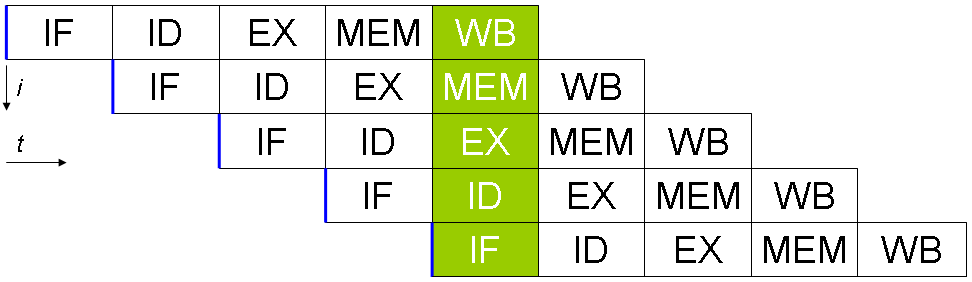
\includegraphics[width=8cm]{informatika/operacne_systemy_a_hw/obrazky/Fivestagespipeline.png}
  \end{center}

  \item \textbf{superskalarita}: Dialša možnosť je použitie superscalar designu, ktorý obsahuje dlhú inštrukčnú pipeline a viacero identických execution jednotiek.  
  \begin{center}
  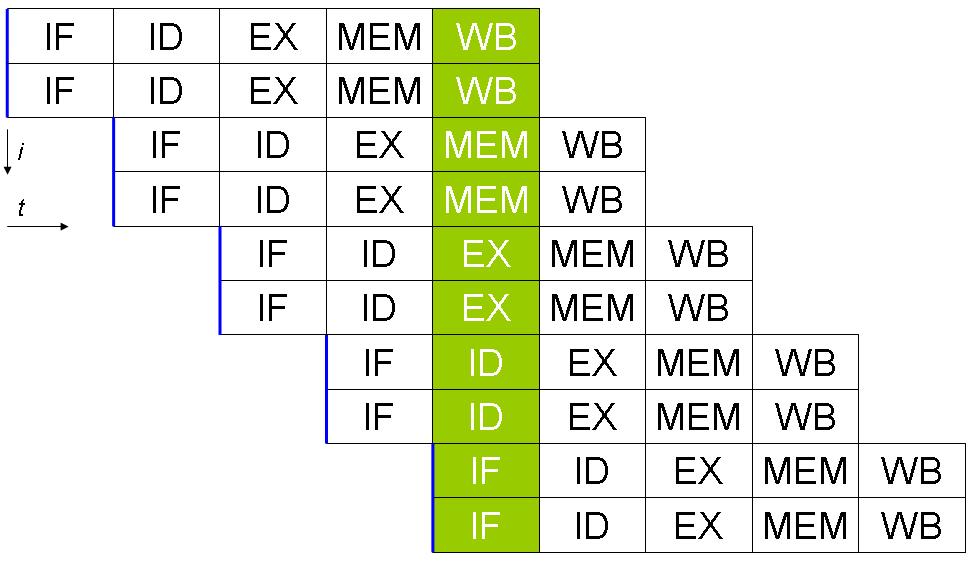
\includegraphics[width=8cm]{informatika/operacne_systemy_a_hw/obrazky/Superscalarpipeline.png}
  \end{center}	

  \item \textbf{Out of order execution}
  \begin{penumerate}
	  \item Načtení instrukce, případně její rozdrobení na mikroinstrukce
	  \item Zařazení do vyčkávací stanice (instruction pool)
	  \item Instrukce čeká na všechny svoje operandy
	  \item Instrukce se vykoná ve své výkonné jednotce (je vybírána z instruction poolu nezávisle na ostatních)
	  \item Výsledky se uchovají ve frontě (reorder buffer)
	  \item Až se všechny starší instrukce zapíší do registrů, zapíše se výsledek této instrukce (opětovné řazení)
  \end{penumerate}

  \item \textbf{Predikce skoků}~-- hluboké pipeliny mají problém, pokud podmíněný skok není proveden; dynamická predicke skoků (historie CPU~-- vzory nějaké hloubky) vs. statická (bez nápovědy~-- skok vpřed se neprovede, skok vzad se provede; s nápovědou~-- překladač odhaduje pravděpodobnost skoku)

  \item \textbf{Spekulativní vykonávaní}~-- vykonávání kódu, který nemusí být zapotřebí; významná disproporce mezi rychlostí CPU a paměti; typické využití je značné předsunutí čtecích operací; CPU provádí i odsouvání zápisových operací


  \item \textbf{Data parallelism}: SIMD inštrukcie (napr. multimediálne inštrukcie), vektorové procesory...
\end{pitemize}
\end{obecne}

\subsubsection*{Multiprocesory}

TODO: jde o copy \& paste z Wiki ... předělat česky/slovensky
\medskip

\begin{definiceN}{Multiprocesor}
  O \emph{multiprocesoru} mluvíme, pokud je použito dvou nebo více procesorů
  (CPU) v rámci jednoho počítačového systému. Termín je také používán mluvíme-li
  o schopnosti systému využívat více procesorů a/nebo schopnosti rozdělovat
  úlohy mezi jednotlivými procesory.
\end{definiceN}

\begin{obecne}{Vztah k datům a instrukcím}
In multiprocessing, the processors can be used to execute a single sequence of instructions in multiple contexts (single-instruction, multiple-data or SIMD, often used in vector processing), multiple sequences of instructions in a single context (multiple-instruction, single-data or MISD, used for redundancy in fail-safe systems and sometimes applied to describe pipelined processors or hyperthreading), or multiple sequences of instructions in multiple contexts (multiple-instruction, multiple-data or MIMD).
\end{obecne}

\begin{obecne}{Symetrie}
In a multiprocessing system, all CPUs may be equal, or some may be reserved for special purposes. A combination of hardware and operating-system software design considerations determine the symmetry (or lack thereof) in a given system. For example, hardware or software considerations may require that only one CPU respond to all hardware interrupts, whereas all other work in the system may be distributed equally among CPUs; or execution of kernel-mode code may be restricted to only one processor (either a specific processor, or only one processor at a time), whereas user-mode code may be executed in any combination of processors. Multiprocessing systems are often easier to design if such restrictions are imposed, but they tend to be less efficient than systems in which all CPUs are utilized equally.

Systems that treat all CPUs equally are called symmetric multiprocessing (SMP) systems. In systems where all CPUs are not equal, system resources may be divided in a number of ways, including asymmetric multiprocessing (ASMP), non-uniform memory access (NUMA) multiprocessing, and clustered multiprocessing (qq.v.).
\end{obecne}

\begin{obecne}{Těsnost spojení multiprocesorů}
\begin{pitemize}
    \item \textbf{Tightly-coupled} multiprocessor systems contain multiple CPUs that are connected at the bus level. These CPUs may have access to a central shared memory (SMP or UMA), or may participate in a memory hierarchy with both local and shared memory (NUMA). The IBM p690 Regatta is an example of a high end SMP system. Intel Xeon processors dominated the multiprocessor market for business PCs and were the only x86 option till the release of AMD's Opteron range of processors in 2004. Both ranges of processors had their own onboard cache but provided access to shared memory; the Xeon processors via a common pipe and the Opteron processors via independent pathways to the system RAM.

    \item \textbf{Chip multiprocessors}, also known as multi-core computing, involves more than one processor placed on a single chip and can be thought of the most extreme form of tightly-coupled multiprocessing. Mainframe systems with multiple processors are often tightly-coupled.

    \item \textbf{Loosely-coupled multiprocessor} systems (often referred to as clusters) are based on multiple standalone single or dual processor commodity computers interconnected via a high speed communication system (Gigabit Ethernet is common). A Linux Beowulf cluster is an example of a loosely-coupled system.
\end{pitemize}
Tightly-coupled systems perform better and are physically smaller than loosely-coupled systems, but have historically required greater initial investments and may depreciate rapidly; nodes in a loosely-coupled system are usually inexpensive commodity computers and can be recycled as independent machines upon retirement from the cluster.

\textbf{SMP} (Symmetric Multiprocessing): viac procesorov so zdieľanou operačnou pamäťou (nutné mechanizmy na zabránenie nesprávnych náhľadov na pamäť a migráciu procesov medzi procesormi). SMP systems allow any processor to work on any task no matter where the data for that task are located in memory; with proper operating system support, SMP systems can easily move tasks between processors to balance the workload efficiently.
\end{obecne}

\subsection{Vstupní a výstupní zařízení}

K I/O zařízením je možné přistupovat dvěma způsoby: pomocí \textbf{port}ů (speciální adresový port CPU) nebo \textbf{pamětovým mapováním} (namapování do fyzické paměti).

Zařízení mají různé charakteristiky:
\begin{pitemize}
	\item \textbf{druh}~-- blokové (disk, síťová karta), znakové (klávesnice, myš)
	\item \textbf{přístup}~-- sekvenční (datová páska), náhodný (hdd, cd)
	\item \textbf{komunikace}~-- synchronní (pracuje s daty na žádost~-- disk), asynchronní (\uv{nevyžádaná} data~-- síťová karta)
	\item \textbf{sdílení}~-- sdílené (preemptivní, lze odebrat~-- síťová karta (po multiplexu OS)), vyhrazené (nepreemptivní~-- tiskárna, sdílení se realizuje přes \emph{spooling}). Reálně se rozdíly stírají.
	\item \textbf{rychlost} (od několika Bps po GBps)
	\item \textbf{směr dat}~-- R/W, R/O (CD-ROM), W/O (tiskárna) 
\end{pitemize}

Přenos dat mezi zařízením a CPU/pamětí:
\begin{pitemize}
	\item \textbf{polling}~-- aktivní čekání na změnu zařízení, přenos provádí CPU
	\item \textbf{přerušení}~-- asynchronní přerušení od zařízení, přenos provádí CPU
	\item \textbf{DMA (Direct Memory Access)}~-- zařízení si samo řídí přístup na sběrnici a přenáší data z/do paměti; po skončení přenosu přerušení (oznámení o dokončení)
\end{pitemize}

Cíle I/O software:
\begin{pitemize}
	\item \textbf{Nezávislost zařízení}~-- programy nemusí dopředu vědět, s jakým přesně zařízením budou pracovat~-- je jedno jestli pracuji se souborem na pevném disku, disketě nebo na CD-ROM
	\item \textbf{Jednotné pojmenování} (na UNIXu /dev)
	\item \textbf{Připojení (mount)}~-- časté u vyměnitelných zařízení (disketa); možné i u pevných zařízení (disk); nutné pro správnou funkci cache OS
	\item \textbf{Obsluha chyb}~-- v mnoha případech oprava bez vědomí uživatele (velmi často způsobeno právě uživatelem)
\end{pitemize}

\subsection{Architektury OS}

\begin{obecne}{Klasická struktura~-- monolitická}
Nejstarší, už IBM 360, Unix, Win., všechny služby uvnitř, prováděny ve chráněném módu, jádro poměrně velké, \uv{údajně} nejrychlejší. Program zavolá službu OS, přes tabulku se zjistí adresa přísl. fce, ta se zavolá a vrátí výsledek.  Nevýhoda: horší údržba -- je-li v programu chyba, může poškodit zbývající části systému, rozšiřování za běhu je komplikované. 
\end{obecne}

\begin{obecne}{Virtuální stroje}
Původní nápad : Virtual Machine pro IBM360 -- oddělit multitasking od OS jako ext. stroj. Nad HW byla další vrstva -- \uv{Virtual Machine} -- měla plánovat, vyrábí pro procesy iluzi holého HW; dneska např. VMWare dělá to samé. Pro IBM360 se dalo použít v kombinaci s CMS (jednoúlohový) i původního OS360 (rychlejší než OS360 na holém HW). 

Dnes: definuji abstraktní stroj, pro něj překládám programy (.NET, Java) $\rightarrow$ přenositelnost, kompatibilita (IBM AS400~-- desítky let), problém~-- pomalé. 
\end{obecne}

\begin{obecne}{Mikrojádro}
snaha aby část běžící v kernel módu byla co nejmenší (třeba jen cca 10 KB), nejnovější, experimentální, často pro Distribuované OS (dnes už nepoužívané), hodně procesů \& komunikace (klient/server), mikrojádro řeší jenom komunikaci. 

Filesystém apod. jsou procesy -- aplikace jim posílají přes jádro požadavky. Jediný komerční OS -- Chorus (ústředny). výhoda: když něco spadne, nepoškodí to zbytek, moduly jdou měnit za běhu, komunikace jde snadno rozšířit na komunikaci po síti. 
\end{obecne}

\begin{obecne}{Architektura WinNT}
  Jádro je poměrně malé (cca 1MB), schopné (pro vyšší vrstvy jsou některé schopnosti skryté), na jeho vzniku se podíleli schopní Unixáři. Byla zde snaha o malou velikost, přenositelnost. Jádro je neutrální vzhledem k vyšším vrstvám, nad ním lze vybudovat různé systémy (Windows subsystém, POSIX, OS/2).

  Rozhraní OS a uživ. programů zajišťuje WinAPI, nad ním se nacházejí různé DLL, mezi kernelem a HW je \uv{hardware abstraction layer}, tj. kernel lze jednoduše upravit pro jiné architektury (Alpha, IA-64).
  Grafické drivery jediné mají přímý přístup k HW (kvůli výkonu), části API (USER, GDI) jsou implementované v jádře, přechod mezi user a kernel režimem zajišťuje ntdll.dll (a je tedy využíván všemi programy). Veškeré služby a aplikace běží v user módu nad jádrem.

  \begin{center}
    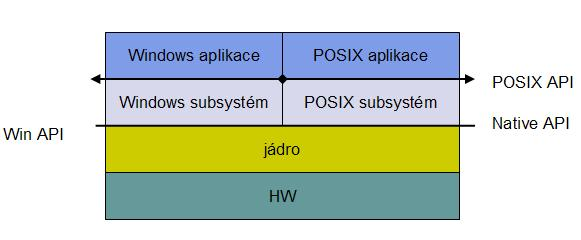
\includegraphics[width=8cm]{informatika/operacne_systemy_a_hw/obrazky/arch-windows.jpg}
  \end{center}
\end{obecne}

\begin{obecne}{Architektura Linuxu}
  \begin{pitemize}
      \item Na úrovni SW -- přenositelnost; abstrakce HW. 
      \item nad HW~-- kernel, nad ním systémová volání, hodně podobné Windows.
  \end{pitemize}

  \begin{center}
    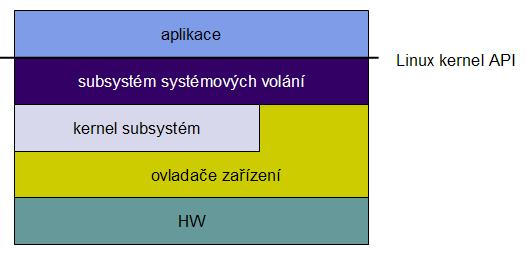
\includegraphics[width=8cm]{informatika/operacne_systemy_a_hw/obrazky/arch-linux.jpg}
  \end{center}
\end{obecne}

\subsection{Procesy, vlákna, plánování}

\subsubsection*{Procesy a vlákna}
Systémové volání je interface mezi OS (kernelspace) a užívatelskými programy (userspace).

\begin{definiceN}{Proces}
  \emph{Proces} je inštancia vykonávaného programu. Kým program je len súbor
  inštrukcií, proces je vlastný \uv{výkon} týchto inštrukcií. Proces má vlastný
  adresný priestor (pamäť), prostriedky, práva a napr. aj ID (Process ID).
\end{definiceN}

Počas života sa môže proces nachádzať v rôznych stavoch:
\begin{pitemize}
  \item \emph{bežiaci}~-- jeden proces na procesor,
  \item \emph{blokovaný}~-- pri použití blokujúceho volania~-- I/O disku atď.,
  \item \emph{pripravený}~-- skončilo blokovanie; spotreboval všetok pridelený čas resp. vrátil riadenie systému, čaká na nové pridelenie procesora,
  \item \emph{zombie}~-- po ukončení procesu, keď už nepracuje~-- ale ešte nebol vymazaný.
\end{pitemize}

\begin{definiceN}{Vlákno}
  \emph{Vlákno} je možnosť pre program ako sa \uv{rozdeliť} na dva alebo viac
  zároveň (resp. pseudo-zároveň) vykonávaných úloh. Oproti procesu mu nie je
  pridelená vlastná pamäť~-- je to len miesto vykonávania inštrukcií v programe.
  Oproti procesu sú jeho \uv{atribútmi} len hodnota programového čítača, stav
  registrov CPU a zásobník.
\end{definiceN}

Oproti Windows/Solaris neobsahuje Linux priamu podporu pre vlákna. Miesto toho podporuje procesy (zhodou okolností :-)) zdieľajúce pamäť. V samotnom jadre linuxu ale vlákna existujú (kthreads).

\subsubsection*{Plánovanie}

Prideľovanie procesorového času jednotlivým procesom má na starosti \emph{plánovač}. Plánovanie pritom môže byť preemptívne alebo nepreemptívne (kooperatívne~-- alla Win16).

\begin{obecne}{Ciele plánovania (niektoré z nich sú očividne protichodné):}
\begin{pitemize}
	\item Spravodlivosť (každy procesor dostane adekvátnu časť času CPU)
	\item Efektívnosť (plne vyťažený procesor)
	\item Minimálna doba odpovede
	\item Průchodnost (maximálny počet spracovaných procesov)
	\item Minimálna réžia systému
\end{pitemize}
\end{obecne}

\begin{obecne}{Kritériá plánovania:}
\begin{pitemize}
	\item Viazanosť procesu na dané CPU a I/O (presun procesu na iný procesor zaberie veľa prostriedkov)
	\item Proces je dávkovy/interaktívny?
	\item Priorita procesu (statická (nemenná~-- okrem \uv{renice}) + dynamická, ktorá sa mení v čase kvôli spravodlivosti)
	\item Ako často proces generuje výpadky stránok (nejaký popis???)
	\item Kolik skutočného času CPU proces obdržel
\end{pitemize}
\end{obecne}

\begin{obecne}{Algoritmy:}
\begin{pitemize}
	\item \textbf{FIFO}: nepreemptívny, proces opustí procesor až po skončení

	\item \textbf{Round Robin}: preemptívne rozšírenie FIFO, po skončení časového kvanta je proces presunutý na koniec fronty

	\item \textbf{Plánovanie s viacerými frontami}: niekoľko front, procesu z $i$-tej fronty je pridelený procesor až keď vo frontách $1, \dots, i-1$ nie je pripravený ziadny proces. Ak proces skončil I/O operáciou, je blokovaný a presunutý do fronty $i-1$, ak skončil preempciou, je pripravený a presunutý do fronty $i+1$.

	\item \textbf{SMP}: fronta CPU čakajúcich na pripravené procesy (aktívne (spotrebováva energiu) vs. pasívne čakanie (špeciálne inštrukcie)), \uv{vzťah}/afinita procesov k CPU

	\item TODO: Plánovanie windows vs. linux???
\end{pitemize}
\end{obecne}

\subsection{Synchronizační primitiva, vzájemné vyloučení}

\subsubsection*{Pojmy}

\emph{Race conditions}: výsledek operace závisí na plánování

\emph{Vzájemné vyloučení (mutual exclusion)}: kritickou operaci provádí nejvýše jeden proces. Podmínky vzájemného vyloučení:
\begin{penumerate}
	\item Žádné dva procesy nemohou být najednou ve stejné kritické sekci
	\item Nemohou být učiněny žádné předpoklady o rychlosti nebo počtu CPU
	\item Žádný proces mimo kritickou sekci nesmí blokovat jiný proces
	\item Žádný proces nesmí čekat nekonečně dlouho v kritické sekci
\end{penumerate}

\emph{Kritická sekce}: část programu, kde se provádí kritická operace

Metody dosáhnutí vzájemného vyloučení: aktivní čekání (busy waiting) a pasivní čekání/blokování.

\subsubsection*{Aktivní čekání}
\emph{Vlastnosti}: spotřebovává čas procesoru, vhodnější pro předpokládané krátké doby čekání, nespotřebovává prostředky OS, rychlejší.

Je možné použít např. \emph{zakázání přerušení} (vhodné pro jádro OS). Používání \emph{zámků} nefunguje:
\begin{verbatim}
int lock;
void proc(void) {
  for (;;) {
    nekritická_sekce();
    while (lock != 0);
    lock = 1;
    kritická_sekce();
    lock = 0;
  }
}
\end{verbatim}
ale \emph{důsledné střídání} ano (to ale porušuje podmínku 3.)

\begin{verbatim}
int turn = 0;

void p1(void)                void p2(void)
{                            {
  for (;;) {                   for (;;) {
    while (turn != 0);           while (turn != 1);
    kritická_sekce();            kritická_sekce();
    turn = 1;                    turn = 0;
    nekritická_sekce();          nekritická_sekce();
  }                            }
}                            }
\end{verbatim}

\emph{Petersonovo řešení}:
\begin{verbatim}
#define N 2                   /* počet procesů */
 
int turn;
int interested[N];            /* kdo má zájem */
 
void enter_region(int proc) { /* proc: kdo vstupuje */
int other;
 
  other = 1-proc;             /* číslo opačného procesu */
  interested[proc] = TRUE;    /* mám zájem o vstup */
  turn = proc;                /* nastav příznak */
  while (turn == proc && interested[other] == TRUE);
}
 
void leave_region(int proc) { /* proc: kdo vystupuje */
  interested[proc] = FALSE;   /* už odcházím */
}
\end{verbatim}
 
\emph{Instrukce TSL} (spin-lock) - je nutné aby ji podporoval HW (všechny současné procesory nějakou mají):
\begin{verbatim}
enter_region:
    tsl   R,lock           ; načti zámek do registru R a
                           ; nastav zámek na 1
    cmp   R,#0             ; byl zámek nulový?
    jnz   enter_region     ; byl-li nenulový, znova
    ret                    ; návrat k volajícímu - vstup do
                           ; kritické sekce
 leave_region:
    mov   lock,#0          ; ulož do zámku 0
    ret                    ; návrat k volajícímu
\end{verbatim}

\subsubsection*{Pasivní čekání}
\emph{Vlastnosti}: proces je ve stavu blokován, vhodné pro delší doby čekání, spotřebovává prostředky OS, pomalejší.

Postup používající Sleep/Wakeup (implementovány OS, atomické operace - sleep uspí volající proces, wakeup probudí udaný proces) nefunguje (viď Problém producent/konzument).

\textbf{Semafory}... Sémantika:
\begin{verbatim}
Down(Semaphore s) {
  wait until s > 0, then s := s-1;
  /* must be atomic once s > 0 is detected */
}
\end{verbatim}
(pokud je čítač $>$ 0, sníží čítač o 1 a pokračuje dál; pokud je čítač $=$ 0, operace DOWN se zablokuje a proces je přidán do fronty čekající na tomto semaforu)

\begin{verbatim}
Up(Semaphore s) {
  s := s+1;   /* must be atomic */
}
\end{verbatim}
(pokud je fronta neprázdná, vybere libovolný proces a ten probudí za DOWN; jinak zvětší čítač o 1)

\begin{verbatim}
Init(Semaphore s, Integer v) {
  s := v;
}
\end{verbatim}

Je možné \uv{používať} aj sémantiku, kde sa hodnota vždy zníži/zvýši o 1 (a je možné sa teda dostať do záporných hodnôt semafóru)... Špeciálny (binárny) typ semaforu, kde sú povolené len hodnoty 0 a 1 (v Up sa miesto $s:=s+1$ volá $s:=1$) sa nazýva \emph{mutex} a používa sa na riadenie prístupu k jednej premennej.

\textbf{Monitory}
\par Implementovány překladačem, lze si představit jako třídu C++ (všechny proměnné privátní, funkce mohou být i veřejné), vzájemné vyloučení v jedné instanci (zajištěno synchronizací na vstupu a výstupu do/z veřejných funkcí, synchronizace implementována blokovacím primitivem OS). ???TODO

\textbf{Zprávy}
\par Operace SEND a RECEIVE, zablokování odesílatele/příjemce, adresace proces/mailbox, rendez-vous...

\textbf{RWL - read-write lock}, \textbf{bariéry}...

Ekvivalence primitiv - pomocí jednoho blokovacího primitiva lze implementovat jiné blokovací primitivum.

Rozdíly mezi platformami: Windows - jednotné funkce pro pasivní čekání, čekání na více primitiv, timeouty. Unix - OS implementuje semafor, knihovna pthread.

\subsubsection*{Klasické synchronizační problémy}
\textbf{Problém producent/konzument}
\par Producent vyrába predmety, konzument ich spotrebúva. Medzi nimi je sklad pevnej veľkosti (N). Konzument nemá čo spotrebúvať ak je sklad prázdny; producent prestane vyrábať, ak je sklad plný. 

\begin{verbatim}
int N = 100;
int count = 0;
void producer(void) {
    int item;
    while(TRUE) {
        produce_item(&item);
        if(count==N) sleep ();
        enter_item(item);
        count++;
        if(count == 1) wake(consumer);
    }
}
void consumer(void) {
    int item;
    while(TRUE) {
        if(count==0) sleep ();
        remove_item(&item);
        count--;
        if(count==N-1)
            wake(producer);
        consume_item(&item);
    }
}
\end{verbatim}

\begin{penumerate}
	\item Buffer je prázdny, a konzument práve prečítal count, aby zistil, či je rovný nule
	\item Preplánovanie na producenta
	\item Producent vytvorí item a zvýši count
	\item Producent zistí, či je count rovný jednej. Zistí že áno, čo znamená že konzument bol predtým zablokovaný (pretože muselo byť 0), a zavolá wakeup
	\item Teraz môže dôjsť k zablokovaniu: konzument sa uspí, pretože si myslí, že nemá čo zobrať; producent bude chvíľu produkovať a dôjde "preplneniu" $\Rightarrow$ uspí sa; spí producent aj konzument :o) 
\end{penumerate}

\textbf{Problém obědvajících filosofů}
\par Pět filosofů sedí okolo kulatého stolu. Každý filosof má před sebou talíř špaget a jednu vidličku. Špagety jsou bohužel slizké a je třeba je jíst dvěma vidličkami. Život filosofa sestává z období jídla a období přemýšlení. Když dostane hlad, pokusí se vzít dvě vidličky, když se mu to podaří, nají se a vidličky odloží.

\textbf{Problém ospalého holiče}
\par Holič má ve své oficíně křeslo na holení zákazníka a pevný počet sedaček pro čekající zákazníky. Pokud v oficíně nikdo není, holič se posadí a spí. Pokud přijde první zákazník a holič spí, probudí se a posadí si zákazníka do křesla. Pokud přijde zákazník a holič už střihá a je volné místo v čekárně, posadí se, jinak odejde.

\subsection{Zablokování a zotavení z něj}

Prostředek je cokoliv, k čemu je potřeba hlídat přístup (HW zařízení~-- tiskárny, cpu; informace~-- záznamy v DB). Je možné je rozdělit na \emph{odnímatelné} (lze odejmout procesu bez následků~-- CPU, paměť) a \emph{neodnímatelné} (nelze odejmnout bez nebezpečí selhání výpočtu~-- CD-ROM, tiskárna... tento druh způsobuje problémy).

Práce s prostředky probíhá v několika krocích: \emph{žádost o prostředek} (blokující, právě tady dochází k zablokování), \emph{používání} (např. tisk), \emph{odevzdání} (dobrovolné/při skončení procesu).

Množina procesů je \emph{zablokována}, jestliže každý proces z této množiny čeká na událost, kterou může způsobit pouze jiný proces z této množiny.

\subsubsection*{Coffmanovy podmínky}
Splnenie týchto podmienok je nutné pre zablokovanie:
\begin{penumerate}
	\item \textbf{Vzájemné vyloučení} – každý prostředek je buď vlastněn právě jedním procesem nebo je volný.
	\item \textbf{Drž a čekej} – procesy aktuálně vlastnící nějaké prostředky mohou žádat o další.
	\item \textbf{Neodnímatelnost} – přidělené prostředky nemohou být procesům odebrány.
	\item \textbf{Čekání do kruhu} – existuje kruhový řetěz procesů, kde každý z nich čeká na prostředek vlastněný dalším článkem řetězu.
\end{penumerate}

\subsubsection*{Řešení zablokování}
\begin{pitemize}
	\item \textbf{Pštrosí algoritmus}~-- Zablokování se ani nedetekuje, ani se mu nezabraňuje, ani se neodstraňuje, Uživatel sám rozhodne o řešení (kill). Nespotřebovává prostředky OS~-- nemá režii ani neomezuje podmínky provozu. (Nejčastější řešení~-- Unix, Windows) 
	\item \textbf{Detekce a zotavení}~-- Hledá kružnici v orientovaném grafu (hrany vedou od procesu, který čeká, k procesu, který prostředek vlastní), pokud tam je kružnice, nastalo zablokování a je třeba ho řešit:
		\begin{pitemize}
			\item \emph{Odebrání prostředku}~-- dohled operátora, pouze na přechodnou dobu
			\item \emph{Zabíjení procesů z cyklu} (resp. mimo cyklus vlastnící identický prostředek)
			\item \emph{Rollback} (OS ukládá stav procesů, při zablokování se některé procesy vrátí do předchozího stavu $\Rightarrow$ ztracena práce... obdoba u DB)
		\end{pitemize}
	\item \textbf{Vyhýbání se}~-- Bezpečný stav (procesy/prostředky nejsou zablokovány, existuje cesta, jak uspokojit všechny požadavky na prostředky spouštěním procesů v jistém pořadí); Viď. bankéřův algoritmus. Nutné je předem znát všechny prostředky, které budou programy potřebovat; OS pak dává prostředky tomu, který je nejblíž svému maximu potřeby a navíc pro který je prostředků dost na dokončení. Dnes se moc nepoužívá.
	\item \textbf{Předcházení (prevence)}~-- napadení jedné z Coffmanovy podmínek
		\begin{penumerate}
			\item \emph{Vzájemné vyloučení}~-- \emph{spooling} (prostriedky spravuje jeden systemový proces, ktory dohliada na to, aby jeho stav bol konzistentny (tiskarna)~-- pozor na místo na disku)
			\item \emph{Drž a čekej}~-- žádat o všechny prostředky před startem procesu. Nejprve všechno uvolnit a pak znovu žádat o všechny najednou
			\item \emph{Neodnímatelnost}~-- vede k chaosu
			\item \emph{Čekání do kruhu}~-- nejvýše jeden prostředek~-- všechny prostředky jednoznačně očíslovány, procesy mohou žádat o prostředky jen ve vzestupném pořadí

		\end{penumerate}
			\item \emph{Dvojfázové zamykání}~-- nejprve postupně všechno zamykám (první fáze). Potom se může pracovat se zamčenými prostředky~-- a na závěr se už jen odemyká (druhá fáze)~-- viď transakční spracování u databází ((striktní/konzervativní) dvoufázové zpracování)
\end{pitemize}

\textbf{Bankéřův algoritmus}: Bankéř má klienty a těm slíbil jistou výšku úvěru. Bankéř ví, že ne všichni klienti potřebují plnou výši úvěru najednou. Klienti občas navštíví banku a žádají postupně o prostředky do maximální výšky úvěru. Až klient skončí s obchodem, vrátí bance vypůjčené peníze. Bankéř peníze půjčí pouze tehdy, zůstane-li banka v bezpečném stavu.

\subsection{Organizace paměti, alokační algoritmy}

\textbf{Hierarchie paměti} (směrem odshora dolů roste velikost, cena na bajt a rychlost klesá~-- a naopak\dots):
\begin{pitemize}
    \item \emph{registry CPU} --- 10ky-100vky bajtů (IA-32: obecné registy pár 10tek), IA-64~-- až kB (extrém), stejně rychlé jako CPU. 
    \item \emph{cache} --- z pohledu aplikací není přímo adresovatelná; dnes řádově MB, rozdělení podle účelu, několik vrstev. L1 cache (cca 10ky kB)~-- dělené instrukce/data; L2 (cca MB) sdílené instr\&data, běží na rychlosti CPU (dřív bývala pomalejší), servery~-- L3 (cca 10MB). Vyrovnává rozdíl rychlosti CPU a RAM. Využívá lokality programů -- cyklení na místě; sekvenčního přístupu k datům. Pokud nenajdu co chci v cache -- \uv{cache-miss}, načítá se potřebné z RAM (po blocích), jinak (v 95-7\% případů) nastane \uv{cache-hit}, tj. požadovaná data v cache opravdu jsou a do RAM nemusím.
    \item \emph{hlavní paměť} (RAM) --- přímo adresovatelná procesorem, 100MB~-- GB; pomalejší než CPU; CAS~-- doba přístupu na urč. místo~-- nejvíc zdržuje (v 1 sloupci už čte rychle, dat. tok dostatečný), další~-- latence~-- doba než data dotečou do CPU~-- hraje roli vzdálenost (AMD- integrovaný řadič v CPU) 
    \item \emph{pomocná paměť} --- není přímo adresovatelná, typicky HDD; náh. přístup, ale pomalejší. ~100GB, různé druhy~-- IDE, SATA, SCSI; nejvíc zdržuje přístupová doba (čas seeku) cca 2-10ms; obvykle sektor~-- 512 B; roli hraje i rychlost otáčení (4200~-- 15000 RPM)~-- taky řádově ms. 
    \item \emph{zálohovací paměť} --- nejpomalejší, z teorie největší, dnes ale neplatí; typicky~-- pásky; pro větší kapacitu~-- autoloadery ; sekvenční přístup; dnes~-- kvůli rychlosti často zálohování RAIDem.
\end{pitemize}

\textbf{Správce paměti}: část OS, která spravuje paměťovou hierarchii se nazývá\\správce paměti (memory manager):
\begin{pitemize}
	\item udržuje informace o volné/plné části paměti
	\item stará se o přidělování paměti
	\item a \uv{výměnu paměti s diskem}
\end{pitemize}

\textbf{Přiřazení adresy}
\begin{pitemize}
	\item při překladu (je již známo umístění procesu, generuje se absolutní kód, PS: statické linkování)
	\item při zavádění (OS rozhodne o umístění~-- generuje se kód s relokacemi, PS: dynamické linkování)
	\item za běhu (proces se může stěhovat i za běhu, relokační registr)
\end{pitemize}

\textbf{Overlay}~-- Proces potřebuje více paměti než je skutečně k dispozici.
Programátor tedy rozdělí program na nezávislé části (které s v paměti podle
potřeby vyměňnují) a část nezbytnou pro všechny části\dots

\textbf{Výměna (swapping)}~-- dělá se, protože proces musí být v hlavní paměti,
aby jeho instrukce mohly být vykonávány procesorem... Jde o výměnu obsahu paměti
mezi hlavní a záložní.

\textbf{Překlad adresy}~-- nutný, protože proces pracuje v logickém (virtuálním) adresovém prostoru, ale HW pracuje s fyzickým adresovým prostorem...

\textbf{Spojité přidělování}~-- přidělení jednoho bloku / více pamětových oddílů (\emph{pevně}~-- paměť pevně rozdělena na části pro různé velikosti bloků/\emph{volně}~-- v libovolné části volné paměti může být alokován libovolně veliký blok)

\textbf{Informace o obsazení paměti}~-- bitová mapa / spojový seznam volných bloků (spojování uvolněného bloku se sousedy)

\textbf{Alokační algoritmy}:
\begin{pitemize}
	\item \emph{First-fit}~-- první volný dostatečné velikosti~-- rychlý, občas ale rozdělí velkou díru
	\item \emph{Next-fit}~-- další volný dostatečné velikosti~-- jako First-fit, ale rychlejší
	\item \emph{Best-fit}~-- nejmenší volný dostatečné velikosti~-- pomalý (prohledává celý seznam), zanechává malinké díry (ale nechává velké díry vcelku)
	\item \emph{Worst-fit}~-- největší volný~-- pomalý (prohledává celý seznam), rozdělí velké díry
	\item \emph{Buddy systém}~-- paměť rozdělena na bloky o velikosti $2^n$, bloky stejné velikosti v seznamu, při přidělení zaokrouhlit na nejbližší $2^n$, pokud není volný, rozštípnou se větší bloky na příslušné menší velikosti, při uvolnění paměti se slučují sousední bloky (buddy)
\end{pitemize}

\textbf{Fragmentace paměti}:
\begin{pitemize}
	\item \emph{externí}~-- volný prostor rozdělen na malé kousky, pravidlo 50\% -- po nějaké době běhu programu bude cca 50\% paměti fragmentováno a u toho to zůstává
	\item \emph{interní}~-- nevyužití celého přiděleného prostoru
	\item \emph{sesypání}~-- pouze při přiřazení adresy za běhu, nebo segmentaci~-- nelze při statickém přidělení adresy
\end{pitemize}

\subsection{Principy virtuální paměti, stránkování, algoritmy pro výměnu stránek, výpadek stránky, stránkovací tabulky, segmentace}

\subsubsection*{Virtuální paměť}
\begin{pitemize}
	\item procesy pracují s virtuální adresou
	\item mapování adresy na fyzickou - mapovací tabulky
	\item obraz virtuální paměti (VAP) částečně v RAM a částečně na disku
	\item dříve iluze větší paměti, dnes hlavně ochrana přístupu
	\item stránkování / segmentace 
\end{pitemize}

\subsubsection*{Stránkování}
podporované všemi velkými CPU a OS, jednorozměrný VAP
\begin{pitemize}
	\item VAP rozdělen na stránky (velikost je mocnina 2), FAP na rámce (úseky stejné délky)
	\item převod stránkovací tabulkou, příznak existence mapování (výpadek stránky $\rightarrow$ synchronní přerušení)
		\par \begin{center}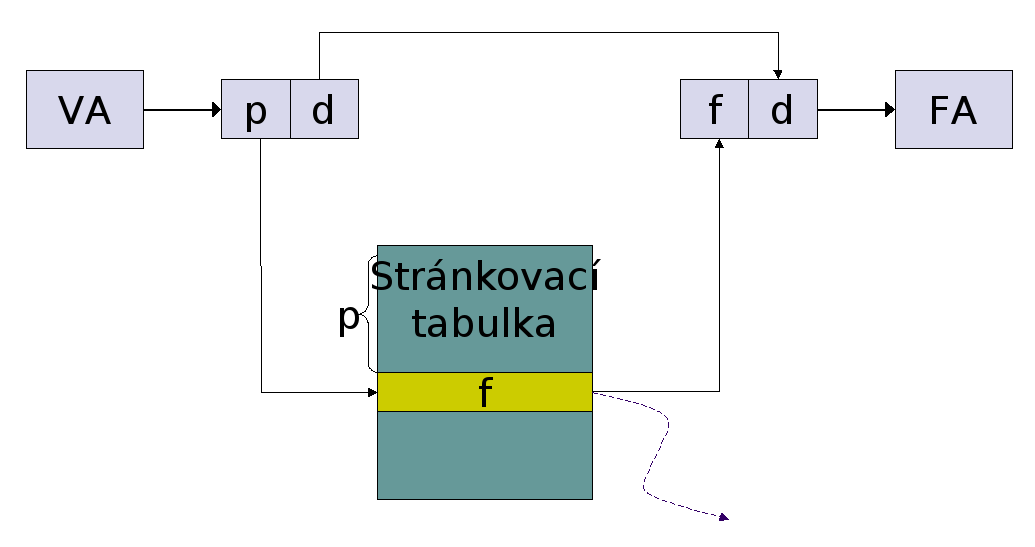
\includegraphics[width=10cm]{informatika/operacne_systemy_a_hw/obrazky/strankovani1.png}\end{center}
	\item umožnuje \emph{oddělené VAP} i \emph{sdílenou paměť} - mapování virtuální stránky 2 procesů na jednu fyzickou
	\item víceúrovňové stránkování (např. kvůli velikosti)
		\par \begin{center} 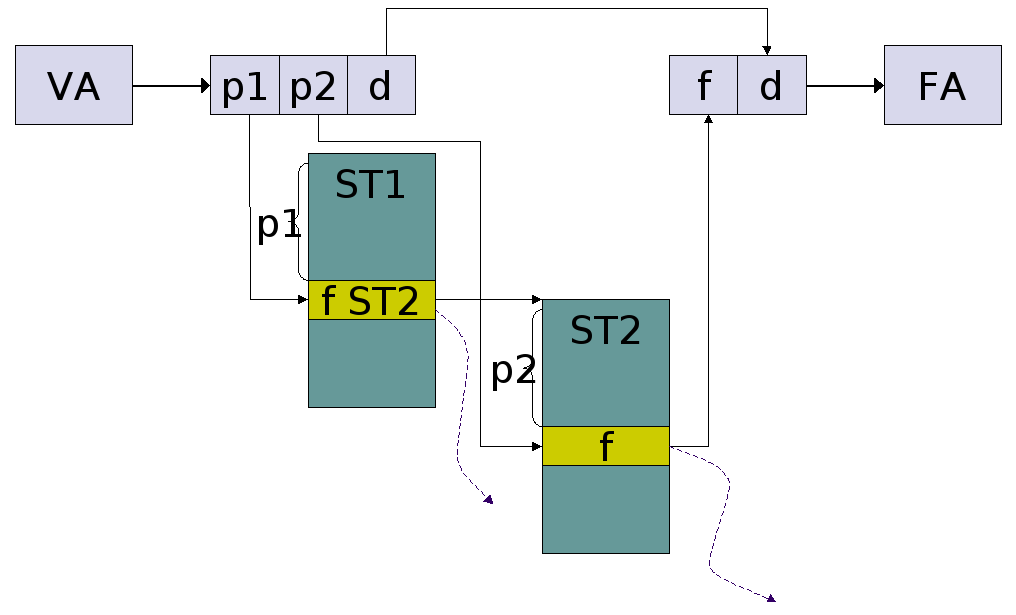
\includegraphics[width=10cm]{informatika/operacne_systemy_a_hw/obrazky/strankovani2.png} \end{center}
	\item TLB (Translation Lookaside Buffer) - asociativní paměť sloužící na rychlé vyhledání mapování virtuální stránky na fyzickou, využívá lokalitu chování programů
		\par \begin{center} 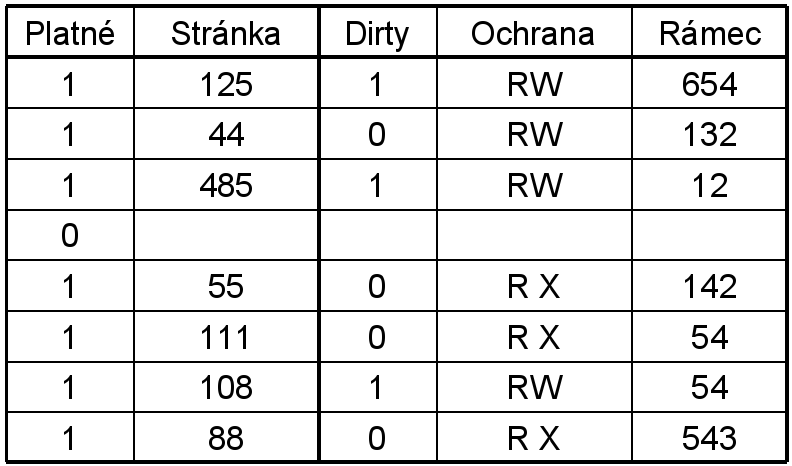
\includegraphics[width=6cm]{informatika/operacne_systemy_a_hw/obrazky/strankovani-tlb.png} \end{center} 
		\par ...nulaúrovňové stránkování - používá pouze TLB, řízeno také OS (oblíbené u 64-bitových CPU - UltraSPARC III)
	\item inverzní stránkování (např. když FAP je menší než VAP, 64-bitové CPU - IA-64)
		\par \begin{center} 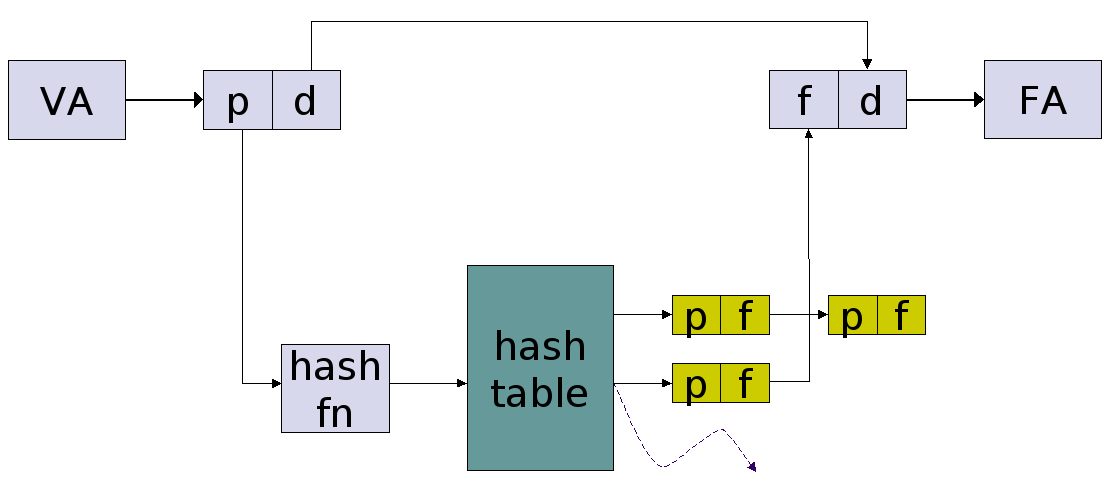
\includegraphics[width=10cm]{informatika/operacne_systemy_a_hw/obrazky/strankovani-inv.png} \end{center} 
\end{pitemize}

Akce vykonávané při výpadku stránky:
\begin{pitemize}
	\item výjimka procesoru
	\item uložit stav CPU (kontext)
	\item zjistit VA
	\item kontrola platnosti adresy a práv
	\item nalezení volného rámce
	\item zrušit mapování na nalezený rámec
	\item pokud je vyhazovaný rámec vyhazován, spustit ukládání na disk
	\item načíst z disku požadovanou stránku do rámce
	\item zavést mapování
	\item obnovit kontext
\end{pitemize}


Při implementaci stránkování je nutno brat v úvahu: 
\begin{pitemize}
    \item \emph{znovuspuštění instrukce} --- je potřeba aby procesor po výpadku zkusil přístup do paměti znova. dnes umí všechny CPU, např. 68xxx - problémy (přerušení v půlce instrukce) 
    \item \emph{sdílení stránek} --- jednomu rámci odp. víc stránek $\rightarrow$ pokud s ním něco dělám, týká se to všech stránek!  musím vše ost. odmapovat. musím si pamatovat mapování pro každý rámec - obrácené tabulky. 
    \item \emph{odstranění položky z TLB při rušení mapování} --- nestačí změnit tabulky, musí se vyhodit i z TLB (kde to může, ale nemusí být). problém - u multiprocesorů má každá CPU vlastní TLB, tabulky jsou sdílené $\rightarrow$ CPU při rušení mapování musí poslat interrupt s rozkazem ke smazání všem (i sobě), počkat na potvrzení akce od všech.
\end{pitemize}

\subsubsection*{Algoritmy pro výměnu stránek}
\begin{pitemize}
	\item \textbf{Optimální stránka} (v okamžiku výpadku stránky vybírám stránku, na níž se přistoupí za největší počet instrukcí) - nelze implementovat
	\item \textbf{NRU} (Not Recently Used) - každá stránka má příznaky Accessed a Dirty (typicky implementovatelné v HW, možno simulovat SW); jednou za čas se smažou všechna A; při výpadku rozdělím stránky podle A,D a vyberu stránku z nejnižší neprázdné třídy:
		\par \begin{center}
		\begin{tabular}{|c|c|c|}
			\hline 
			  & A & D \\
			\hline
			0 & 0 & 0 \\
			\hline
			1 & 0 & 1 \\
			\hline
			2 & 1 & 0 \\
			\hline
			3 & 1 & 1 \\
			\hline
		\end{tabular}
		\end{center}
	\item \textbf{FIFO} (vykazuje anomálie - Belady (zvětšení počtu výpadků stránky, když zvýšíme počet stránek v paměti)), druhá šance (úprava FIFO; pokud A=1, zařadím na konec FIFO... nevykazuje anomálie)
	\item \textbf{Hodiny} - modifikace druhé šance: kruhový zoznam stránek + iterátor na ukazující na nejstarší stránku v zoznamu. Při výpadku (a neexistenci volého rámce) se zjistí, jestli má *iterator nastavený příznak Accessed. Jestli ne, tato stránka bude nahrazena - v opačném případě se Accessed příznak zruší a iterator++. Toto se opakuje, dokud nedojde k výměně\dots
	\item \textbf{LRU} (Least Recently Used) - často používané stránky v posledním krátkém časovém úšeku budou znovu použity, čítač použití stránek, možné implementovat v HW
	\item \textbf{NFU} (Not Frequently Used) - SW simulace LRU, SW čítač ke každé stránce; jednou za čas projdu všechna A a přičtu je k odpovídajícím čítačům; vybírám stránku s nejnižším čítačem; nezapomíná - je možná modifikace se stárnutím čítače
\end{pitemize}

\subsubsection*{Segmentace}
dnes pouze Intel IA-32, dvojrozměrný VAP
\begin{pitemize}
	\item rozdělení programu na segmenty (napr. podle částí s různými vlastnostmi - kód, data, zásobníky\dots), různé délky segmentů, ktoré můžou měnit svoji délku za běhu
	\item VAP dvourozměrný (segment, offset), FAP jednorozměrný (vyzerá jako při spojitém pridělování paměti)
	\item segmentová převodní tabulka (VA se skládá ze dvou častí S:D, v tabulce se najde adresa segmentu S\dots k této adrese se poté přičte D, co je umístnění adresy v FA), příznak existence mapování
	\item při výpadku je nutné měnit celý segment (ty mohou být velké), je možné segmenty sesypat - ale nelze mít segment větší než FAP
\end{pitemize}

Segmentaci je možné kombinovat se stránkováním (odstraňuje nevýhody segmentace, neprovádí se výpadky segmentů):
\par \begin{center}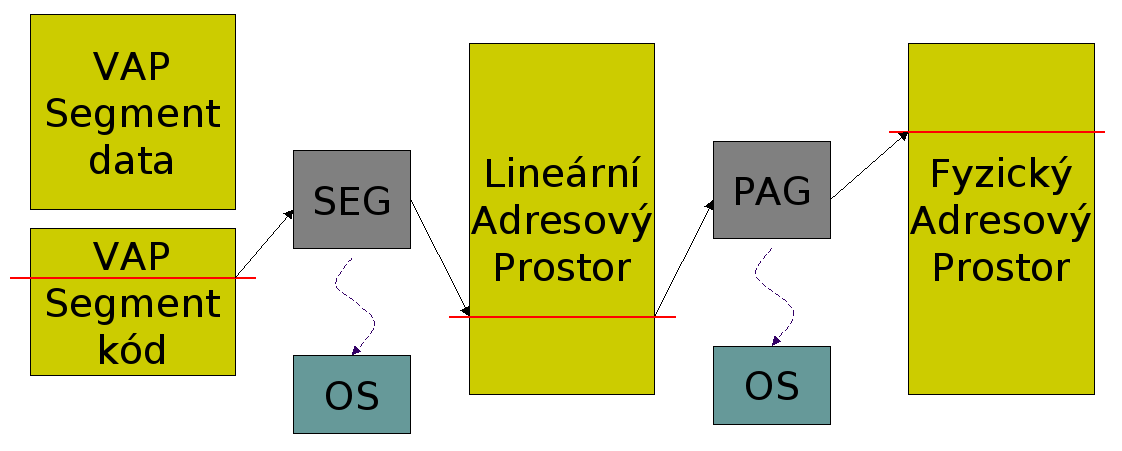
\includegraphics[width=12cm]{informatika/operacne_systemy_a_hw/obrazky/segmentace-a-strankovani.png}\end{center}

\subsection{Systémy souborů, adresářové struktury}

\begin{definiceN}{soubor}
  \emph{Soubor} je pojmenovaná množina souvisejících informací, která leží v
  pomocné paměti (na disku).\\
  \emph{Soubor} je abstrakce, která umožňuje uložit informaci na disk a později ji
  přečíst. Abstrakce odstiňuje uživatele od podrobností práce s disky.
\end{definiceN}

\begin{obecne}{Soubory}
  \begin{pitemize}
    \item pojmenování souboru (umožňuje uživateli přístup k jeho datům;
    přesná pravidla pojmenování určuje OS - malá vs. velká písmenka,
    speciální znaky, délka jména, přípony a jejich význam)
    \item atributy souborů (opět určuje OS) - jméno, typ, umístění, velikost, ochrana, časy, vlastník, \dots
    \item struktura souborů - sekvence bajtů / sekvence záznamů / strom
    \item typy souborů - běžné soubory, adresáře (systémové soubory vytvářející strukturu souborového systému), speciální soubory (znakové/blokové, soft linky)
    \item přístup 
    \begin{pitemize}
      \item \textbf{sekvenční}~-- pohyb pouze vpřed, OS může přednačítat
      \item \textbf{náhodný}~-- možno měnit aktuální pozici
      \item \textbf{paměťově mapované soubory}~-- pojmenovaná virtuální paměť,
      práce se souborem instrukcemi pro práci s pamětí, ušetří se kopírování
      pamětí; mají i problémy (přesná velikost souboru, zvětšování souboru,
      velikost souborů)
    \end{pitemize}
    \item volné místo na disku - bitmapa / spojový seznam volných bloků 
  \end{pitemize}
\end{obecne}

\begin{obecne}{Uložení souborů}
  Soubory se ukládají na disk po blocích
  \begin{pitemize}
    \item souvislá alokace - souvislý sled bloků
    \item spojovaná alokace - blok odkazuje na další
    \item indexová alokace - inode (UNIX) 
  \end{pitemize}
\end{obecne}

\begin{obecne}{Adresáře}
  \begin{pitemize}
    \item zvláštní typ souboru
    \item operace nad adresáři - hledání souboru / vypsání adresáře /
    přejmenování, vytvoření, smazání souboru 
    \item kořen, aktuální adresář, absolutní/relativní cesta
    \item hierarchická struktura 
    \begin{pitemize}
      \item \emph{strom}~-- jednoznačné pojmenování (cesta)
      \item \emph{DAG}~-- víceznačné pojmenování, ale nejsou cykly
      \item \emph{obecný graf}~-- cykly vytváří problém při prohledávání
    \end{pitemize}
    \item implementace adresářů - záznamy pevné velikosti, spojový seznam, B-stromy 
  \end{pitemize}
\end{obecne}

\begin{obecne}{Co musí filesystém umět?}
musí splňovat 3 věci: \emph{správu souborů} (kde jsou, jak velké), \emph{správu adresářů} (převod jméno $\leftrightarrow$ id) (někdy to dělá jiný prostředek, dnes větš. umí FS sám), \emph{správu volného místa}. někdy mohou být i další (odolnost proti výpadkům) 

Velikost bloků -- blok = nejmenší jednotka pro práci s diskem; disk pracuje s min. 1 sektorem (typicky 512 B) - někdy by pak bylo moc bloků $\rightarrow$ OS sdruží několik sektorů lineáně vedle sebe = 1 blok. velikost: velké = rychlejší práce, ale vnitřní fragmentace (průměrný soubor má cca pár KB), malé = malá vnitřní fragmentace, větší režie na info o volném místě/ umístění souboru (zabírá víc bloků!), navíc fragmentace souborů $\rightarrow$ zpomalení. dnes má blok cca 2-4KB.
\end{obecne}

\begin{obecne}{Linky}
  \begin{pitemize}
    \item \textbf{Hard link}~-- Na jedna data souboru se odkazuje z různých položek v adresářích
    \item \textbf{Soft link}~-- Speciální soubor, který obsahuje jméno souboru
  \end{pitemize}
\end{obecne}

\begin{priklady}
  \begin{pitemize}
    \item FAT -- \url{http://en.wikipedia.org/wiki/File\_Allocation\_Table}
    \item NTFS~-- charakteristika, MFT (Master File Table), run list\\\url{http://www.digit-life.com/articles/ntfs/}\\\url{http://www.pcguide.com/ref/hdd/file/ntfs/archSector-c.html}
    \item ext2/ext3~-- struktura, inode, žurnál\\\url{http://www.science.unitn.it/~fiorella/guidelinux/tlk/node95.html}\\\url{http://www.linux-security.cn/ebooks/ulk3-html/0596005652/understandlk-CHP-18.html}
  \end{pitemize}
\end{priklady}

\begin{obecne}{Plánování pohybu hlav disků}
  \begin{pitemize}
    \item FCFS (First-Come, First-Served) - žádné plánování, fronta požadavků, jeden za druhým
    \item SSTF (Shortest Seek Time First) - krajní žádosti mohou "hladovět"
    \item LOOK (výtah), C-LOOK (circular LOOK) - pohyb jen jedním směrem, na konci otočka 
  \end{pitemize}
\end{obecne}

\begin{obecne}{RAID (Redundant Array of Inexpensive Disks)}
  \begin{pitemize}
    \item JBOD (Just a Bunch of Disks)
    \item RAID 0~-- striping, žádná redundance
    \item RAID 1~-- mirroring, redundance
    \item RAID 0+1~-- mirroring a striping
    \item RAID 2~-- 7-bitový paritní Hammingův kód
    \item RAID 3~-- 1 paritní disk, po bitech na disky
    \item RAID 4~-- 1 paritní disk a striping
    \item RAID 5~-- distribuovaná parita a striping
    \item RAID 6~-- distribuovaná parita -- dvojitá P+Q, striping 
  \end{pitemize}
\end{obecne}

\subsection{Bezpečnost, autentifikace, autorizace, přístupová práva}

\begin{definice}
  \begin{pitemize}
    \item \textbf{Ochrana}~-- s prostředky OS mohou pracovat pouze autorizované procesy
    \item \textbf{Autorizace}~-- zjištění oprávněnosti požadavku
    \item \textbf{Bezpečnost}~-- zabraňuje neautorizovaný přístup do systému
    \item \textbf{Právo}~-- povolení/zakázání vykonávat nějakou operaci
    \item \textbf{Doména ochrany}~-- množina párů (objekt:práva)
    \begin{pitemize}
      \item \textbf{ACL (Access Control List)}~-- ke každému objektu seznam práv pro uživatele/skupiny
      \item \textbf{C-list (Capability List)}~-- ke každému uživateli/skupině seznam práv pro objekty
    \end{pitemize}
  \end{pitemize}
\end{definice}

\begin{obecne}{Autentifikace}
  Identifikace něčím, co uživatel ví, má nebo je. 
  \begin{pitemize}
    \item \textbf{Hesla}
    \begin{pitemize}
      \item slovníkový útok (80--90\% hesel je jednoduchých), hrubá síla
      \item vynucování délky a složitosti hesla
    \end{pitemize}
    \item \textbf{Model otázka/odpověď}
    \item \textbf{Fyzický objekt}~-- smartcards, USB klíče
    \item \textbf{Biometrika}~-- otisky prstů, rohovka, hlas
  \end{pitemize}
\end{obecne}

TODO: autorizace, přístupová práva

\subsection{Architektura ISO/OSI}

\subsubsection*{Úvod}
\begin{definice}
\textbf{Síťový model} je ucelená představa o tom, jak mají být sítě řešeny (obsahuje: počet vrstev, co má která vrstva na starosti; neobsahuje: konkrétní představu jak která vrstva plní své úkoly - tedy konkrétní protokoly). Příkladem je \emph{referenční model ISO/OSI} (konkrétní protokoly vznikaly samostatně a dodatečně).
\textbf{Síťová architektura} navíc obsahuje konkrétní protokoly - napr. \emph{rodina protokolů TCP/IP}.
\end{definice}

Referenčný model ISO/OSI (International Standards Organization / Open Systems Interconnection) bol pokusom vytvoriť univerzálnu sieťovú architektúru - ale skončil ako sieťový model (bez protokolov). Pochádza zo \uv{sveta spojov} - organizácie ISO, a bol \uv{oficiálnym riešením}, presadzovaným \uv{orgánmi štátu}; dnes už prakticky odpísaný - prehral v súboji s TCP/IP. ISO/OSI bol reakciou na vznik proprietárnych a uzavretých sietí. Pôvodne mal model popisovať chovanie otvorených systémov vo vnútri aj medzi sebou, ale bolo od toho upustené a nakoniec z modelu ostal len sieťový model (popis funkcionality vrstiev) a konkrétne protokoly pre RM ISO/OSI boli vyvíjané samostatne (a dodatočne zaraďované do rámca ISO/OSI).

Model vznikal maximalistickým spôsobom - obsahoval všetko čo by mohlo byť v budúcnosti potrebné. Vďaka rozsiahlosti štandardu sa implementovali len jeho niektoré podmnožiny - ktoré neboli (vždy) kompatibilné. Vznikol GOSIP (Government OSI Profile) určujúci podmnožinu modelu, ktorú malo mať implementované všetko štátne sieťové vybavenie. Naproti tomu všetkému TCP/IP vzniklo naopak - najprv navrhnutím jednoduchého riešenia, potom postupným obohacovaním o nové vlastnosti (tie boli zahrnuté až po preukázaní \uv{životaschopnosti}).

\subsubsection*{7 vrstev}
Kritériá pri návrhu vrstiev boli napr.: rovnomerná vyťaženosť vrstiev, čo najmenšie dátové toky medzi vrstvami, možnosť prevziať už existujúce štandardy (X.25), odlišné funkcie mali patriť do odlišných vrstiev, funkcie na rovnakom stupni abstrakcie mali patriť do rovnakej vrstvy. Niektoré vrstvy z finálneho návrhu sa používajú málo (relačná a prezentačná), niektoré zase príliš (linková - rozpadla sa na 2 podvrstvy LLC+MAC).

\begin{center}
\begin{tabular}{|c|l|}
	\hline
	aplikační vrstva & vrstvy orientované na podporu aplikací\\
	prezentační vrstva &\\
	relační vrstva &\\
	\hline
	transportní vrstva & přispůsobovací vrstva \\
	\hline
	síťová vrstva & vrstvy orientované na přenos dat\\
	linková vrstva & \\
	fyzická vrstva & \\
	\hline
\end{tabular}
\end{center}

\textbf{Fyzická vrstva} sa zaoberá prenosom bitov (kódovanie, modulácia, synchronizácia...) a ponúka teda služby typu pošli a príjmi bit (pričom neinterpretuje význam týchto dát). Pracuje sa tu s veličinami ako je \emph{šírka pásma}, \emph{modulačná a prenosová rýchlosť}.

\textbf{Linková vrstva} prenáša vždy celé bloky dát (rámce/frames), používa pritom fyzickú vrstvu a prenos vždy funguje len k priamym susedom. Môže pracovať spoľahlivo či nespoľahlivo, prípadne poskytovať QoS/best effort. Ďalej zabezpečuje riadenie toku - zaistenie toho, aby vysielajúci nezahltil príjemcu. Delí sa na dve podvrstvy - MAC (prístup k zdieľanému médiu - rieši konflikty pri viacnásobnom prístupe k médiu) a LLC (ostatné úlohy).  

\textbf{Sieťová vrstva} prenáša pakety (packets) - fakticky ich vkladá do linkových rámcov. Zaručuje doručenie paketov až ku konečnému adresátovi (tj. zabezpečuje smerovanie). Môže používať rôzne algoritmy smerovania - ne/adaptívne, izolované, distribuované, centralizované... (v architektúre TCP/IP je to IP vrstva)

\textbf{Transportná vrstva} zabezpečuje komunikáciu medzi koncovými účastníkmi (end-to-end) a môže meniť nespoľahlivý charakter komunikácie na spoľahlivý, menej spoľahlivý na viac spoľahlivý, nespojovaný prenos na spojovaný... Príkladom sú napr. TCP a UDP. Ďalšou úlohou je rozlišovanie jednotlivých entit (na rozdiel od napr. sieťovej vrstvy) v rámci uzlov - procesy, démony, úlohy (rozlišuje sa zväčša nepriamo - napr. v TCP/IP pomocou portov).

\textbf{Relačná vrstva} zaisťuje vedenie relácií - šifrovanie, synchronizáciu, podporu transakcií. Je to najkritizovanejšia vrstva v ISO/OSI modele, v TCP/IP úplne chýba.

\textbf{Prezentačná vrstva} slúži na konverziu dát, aby obe strany interpretovali dáta rovnako (napr. reálne čísla, rôzne kódovanie textov). Ďalej má na starosti konverziu dát do formátu, ktorý je možné preniesť: napr. linearizácia viacrozmerných polí, dátových štruktúr; konverzia viacbajtových položiek na jednotlivé byty (little vs. big endian). \emph{Poznámka}: Zápis čísla 1234H v Big endian je [12:34:--:--] (sun, motorola), v Little endian [--:--:34:12] (intel, amd, ethernet).

\textbf{Aplikačná vrstva} mala pôvodne obsahovať aplikácie - ale tých je veľa a nebolo možné ich štandardizovať. Teraz teda obsahuje len \uv{jadro} aplikácií - tie, ktoré malo zmysel štandardizovať (email a pod.). Ostatné časti aplikácií (GUI) boli vysunuté nad aplikačnú vrstvu.

\subsubsection*{Kritika}
Model ISO/OSI:
\begin{pitemize}
	\item je príliš zložitý, ťažkopádny a obtiažne implementovateľný
	\item je príliš maximalistický
	\item nerešpektuje požiadavky a realitu bežnej praxe
	\item počítal skôr s rozľahlými sieťami ako s lokálnymi
	\item niektoré činnosti (funkcie) zbytočne opakuje na každej vrstve
	\item jednoznačne uprednostňuje spoľahlivé a spojované prenosové služby (ale tie sú spojené s veľkou réžiou $\Rightarrow$ spoľahlivosť si efektívnejšie zabezpečia koncové uzly)
\end{pitemize}

Možnosť nespoľahlivého/nespojovaného spojenia bolo pridané do štandardu až dodatočne, napriek tomu bol porazený architektúrou TCP/IP. Používajú sa však niektoré prevzaté prokoly - X.400 (elektronická pošta), X.500 (adresárové služby - odľahčením vznikol úspešný protokol LDAP).

\subsection{Rodina protokolů TCP/IP (ARP, IPv4, IPv6, ICMP, UDP, TCP) -- adresace, routing, fragmentace, spolehlivost, flow control, congestion control, NAT}
\begin{center}
\begin{tabular}{|c|c|}
	\hline
	ISO/OSI & TCP/IP \\
	\hline
	\hline
	aplikační vrstva & aplikační vrstva\\
	prezentační vrstva &\\
	relační vrstva &\\
	\hline
	transportní vrstva & transportní vrstva \\
	\hline
	síťová vrstva & síťová vrstva (též IP vrstva) \\
	\hline
	linková vrstva & vrstva síťového rozhraní\\
	fyzická vrstva & \\
	\hline
\end{tabular}
\end{center}

Obvyklé označenie je \emph{TCP/IP protocol suite} (súčasťou je viac ako 100 protokolov). Architektúra vznikla postupne (v akademickom prostredí, neskôr sa rozšírila aj do komerčnej sféry) -- najprv vznikli protokoly, potom vrstvy -- a od vzniku sa toho zmenilo len málo (zmeny sú aditívne). Je to najpoužívanejšia sieťová technológia (IP over everything, everything over IP). Prístup autorov bol, na rozdiel od ISO/OSI, od jednoduchšieho k zložitejšiemu -- najprv sa vytvárajú jednoduché riešenia, ktoré sa postupne obohacujú. Až sa riešenie prakticky overí (2 nezávislé implementácie), vznikne štandard. TCP/IP predpokladá že siete sú typu nespojované, nespoľahlivé a best effort. Všetká inteligencia je sústredená do koncových uzlov, sieť je \uv{hlúpa} ale rýchla.

TCP/IP bol pôvodne určený pre ARPAnet -- nemohol mať teda žiadnu centrálnu časť a musel byť robustný voči chybám (nespoľahlivé/nespojované prenosy). Dôraz sa kládol aj na "internetworking". Nebolo však požadované zabezpečenie, mobilita ani kvalita služieb.

TCP/IP nedefinuje rôzne siete (čo sa hardvérových vlastností týka) a technológie vo vrstve sieťového rozhrania -- iba sa snaží nad nimi prevádzkovať protokol IP (okrem SLIP a PPP pre dvojbodové spoje). V sieťovej vrstve je IP protokol, v transportnej jednotné transportné protokoly (TCP a UDP), v aplikačnej potom jednotné základy aplikácií (email, prenos súborov, remote login...).

\subsubsection*{Adresace, IPv4, IPv6}
Data se v IP síti posílají po blocích nazývaných datagramy. Jednotlivé datagramy putují sítí zcela nezávisle, na začátku komunikace není potřeba navazovat spojení či jinak \uv{připravovat cestu} datům, přestože spolu třeba příslušné stroje nikdy předtím nekomunikovaly.

IP protokol v doručování datagramů poskytuje nespolehlivou službu, označuje se také jako best effort – \uv{nejlepší úsilí}; tj. všechny stroje na trase se datagram snaží podle svých možností poslat blíže k cíli, ale nezaručují prakticky nic. Datagram vůbec nemusí dorazit, může být naopak doručen několikrát a neručí se ani za pořadí doručených paketů. Pokud aplikace potřebuje spolehlivost, je potřeba ji implementovat v jiné vrstvě síťové architektury, typicky protokoly bezprostředně nad IP (viz TCP).

Pokud by síť často ztrácela pakety, měnila jejich pořadí nebo je poškozovala, výkon sítě pozorovaný uživatelem by byl malý. Na druhou stranu příležitostná chyba nemívá pozorovatelný efekt, navíc se obvykle používá vyšší vrstva, která ji automaticky opraví.

V \textbf{IPv4} je \emph{adresou} 32bitové číslo, zapisované po jednotlivých bajtech, oddělených tečkami. Takových čísel existuje celkem $2^{32}$. Určitá část adres je ovšem rezervována pro vnitřní potřeby protokolu a nemohou být přiděleny. Dále pak praktické důvody vedou k tomu, že adresy je nutno přidělovat hierarchicky, takže celý adresní prostor není možné využít beze zbytku. To vede k tomu, že v současnosti je již znatelný nedostatek IP adres, který řeší různými způsoby: dynamickým přidělováním (tzn. např. každý uživatel dial-up připojení dostane dočasnou IP adresu ve chvíli, kdy se připojí, ale jakmile se odpojí, je jeho IP adresa přidělena někomu jinému; při příštím připojení pak může tentýž uživatel dostat úplně jinou adresu), překladem adres (NAT) a podobně. Ke správě tohoto přidělování slouží specializované síťové protokoly, jako např. DHCP.

Pôvodný koncept adries počítal so štruktúrou adresy IPv4 v tvare \emph{sieť:počítač}, kde bolo delenie častí pevne dané. Neskôr sa to ale ukázalo ako príliš hrubé delenie a lokálna časť adresy (v rámci jednej podsiete) može mäť dnes promenlivú dĺžku. Obecne platí, že medzi adresami v rovnakej podsieti (majú rovnakú sieťovú časť) je možné dopravovať dáta priamo -- dotyční účastníci sú prepojení jedným ethernetom alebo inou lokálnou sieťou. V opačnom prípade sa dáta dopravujú \emph{smerovačmi/routermi}. Hranicu v adrese medzi adresou siete a počítača určuje dnes maska podsiete. Jedná sa o 32 bitovú hodnotu, ktorá obsahuje jednotky tam, kde je v adrese určená sieť.

\textbf{Adresovanie sietí} bolo v prvopočiatkoch internetu vyriešené staticky -- prvých 8 bitov adresy určovalo sieť, zvyšok jednotlivé počítače (existovať tak mohlo max. 256 sietí). S nástupom lokálnych sietí bolo tento systém potrebné zmeniť -- zaviedli sa \emph{triedy IP adries}. Existovalo 5 tried (A(začiatok 0, hodnoty prvého bajtu 0-127, maska 255.0.0.0), B(10, 128-191, 255.255.0.0), C(110, 192-223, 255.255.255.0), D(1110, 224-239, určené na multicast) a E(1111, 240-255, určené ako rezerva)). Postupom času sa ale aj toto rozdelenie ukázalo ako nepružné a bol zavedený CIDR (Classless Inter-Domain Routing) systém v ktorom je možné hranicu medzi adresou siete a lokálnou časťou adresy umiestniť ľubovoľne (označuje sa potom ako kombinácia prefixu a dĺžky vo forme 192.168.0.0/24, kde 24 znamená že adresu tvorí prvých 24 bitov -- jiný zápis je pomocí už zmiňované masky podsítě, tj. 192.168.0.0 s maskou 255.255.255.0).

Medzi adresami existujú niektoré tzv. \textbf{vyhradené adresy}, ktoré majú špeciálny význam.
\begin{pitemize}
	\item Adresa s (binárnymi) nulami v časti určujúcej počítač (192.168.0.\textbf{0} (/24)) znamená \uv{táto sieť}, resp. \uv{táto stanica}.
	\item Adresa s jednotkami v časti určujúcej počítač (192.168.0.\textbf{255} (/24)) znamená broadcast -- všesmerové vysielanie.
	\item Adresy 10.0.0.0 -- 10.255.255.255, 172.16.0.0 -- 172.31.255.255 a 192.168.0.0 -- 192.168.255.255 sa používajú na adresovanie interných sietí -- smerovače tieto adresy nesmie smerovať ďalej do internetu.
\end{pitemize}

\textbf{IPv6} je trvalejším riešením nedostatku adries -- zatiaľ sa ale rozširuje veľmi pozvolna. Adresa v IPv6 má dĺžku 128 bitov (oproti 32), čo znamená cca. $6 \times 10^{23}$ IP adries na $1 m^2$ zemského povrchu -- umožňuje teda, aby každé zariadenie na zemi malo vlastnú jednoznačnú adresu. Adresa IPv6 sa zapisuje ako osem skupín po štyroch hexadecimálnych číslach (napr. 2001:0718:1c01:0016:0214:22ff:fec9:0ca5) -- pričom úvodné nuly v číslach je možné vynechať. Ak po sebe nasleduje niekoľko nulových skupín, je možné použiť len znaky :: -- napr. ::1 miesto 0000:0000:.......:0001. Toto je možné použiť len raz v zápise adresy. RFC 4291 zavádza 3 typy adries:
\begin{pitemize}
	\item \textbf{inidividuálne / unicast} -- identifikujú práve jedno rozhranie
	\item \textbf{skupinové / multicast} -- určuje skupinu zariadení, ktorým sa má správa dopraviť
	\item \textbf{výberové / anycast} -- určuje tiež skupinu zariadení, dáta sa však doručia len jednému z členov (najbližšiemu)
\end{pitemize}
IPv6 neobsahuje všesměrové (broadcast) adresy. Byly nahrazeny obecnějším modelem skupinových adres a pro potřeby doručení dat všem zařízením připojeným k určité síti slouží speciální skupinové adresy (např. ff02::1 označuje všechny uzly na dané lince).

IPv6 zavádí také koncepci dosahu (scope) adres. Adresa je jednoznačná vždy jen v rámci svého dosahu. Nejčastější dosah je pochopitelně globální, kdy adresa je jednoznačná v celém Internetu. Kromě toho se často používá dosah linkový, definující jednoznačnou adresu v rámci jedné linky (lokální sítě, např. Ethernetu). Propracovanou strukturu dosahů mají skupinové adresy (viz níže).

Adresní prostor je rozdělen následovně:
\begin{center}
\begin{tabular}{|l|l|}
	\hline
	prefix & význam \\
	\hline
	\hline
	::/128 & neurčená \\
	::1/128 & smyčka (loopback) \\
	ff00::/8 & skupinové \\
	fe80::/10 & individuální lokální linkové \\
	ostatní & individuální globální \\
	\hline
\end{tabular}
\end{center}

Výběrové adresy nemají rezervovánu svou vlastní část adresního prostoru. Jsou promíchány s individuálními a je otázkou lokální konfigurace, aby uzel poznal, zda se jedná o individuální či výběrovou adresu.

Strukturu globálních individuálních IPv6 adres definuje RFC 3587. Je velmi jednoduchá a de facto odpovídá (až na rozměry jednotlivých částí) výše uvedené struktuře IPv4 adresy.

\begin{center}
\begin{tabular}{|l|l|l|}
	\hline
	n bitů & 64-n bitů & 64 bitů \\
	globální směrovací prefix & adresa podsítě & adresa rozhraní \\
	\hline
\end{tabular}
\end{center}

Globální směrovací prefix je de facto totéž co adresa sítě, následuje adresa podsítě a počítače (přesněji síťového rozhraní). V praxi je adresa podsítě až na výjimky 16bitová a globální prefix 48bitový. Ten je pak přidělován obvyklou hierarchií, jejíž stávající pravidla jsou:
\begin{pitemize}
    \item první dva bajty obsahují hodnotu 2001 (psáno v šestnáctkové soustavě)
    \item další dva bajty přiděluje regionální registrátor (RIR)
    \item další dva bajty přiděluje lokální registrátor (LIR)
\end{pitemize}

Reálná struktura globální individuální adresy tedy vypadá následovně:

\begin{center}
\begin{tabular}{|l|l|l|l|l|}
	\hline
	16 bitů & 16 bitů & 16 bitů & 16 bitů & 64 bitů \\
	2001 & přiděluje RIR &přiděluje LIR &adresa podsítě & adresa rozhraní \\
	\hline
\end{tabular}
\end{center}
Adresa rozhraní by pak měla obsahovat modifikovaný EUI-64 identifikátor. Ten získáte z MAC adresy jednoduchým postupem: invertuje se druhý bit MAC adresy a doprostřed se vloží dva bajty obsahující hodnotu fffe. Z ethernetové adresy 00:14:22:c9:0c:a5 tak vznikne identifikátor 0214:22ff:fec9:0ca5.

Adresy začínajúce hodnotou ff sú tzv. "skupinové adresy" -- štyri nasledujúce bity v nej obsahujú príznaky, ďalšie štyri potom dosah (napr. interface-local, link-local, admin-local, site-local, organization-local, global...)

IPv6 ďalej podporuje QoS a bezpečnosť (IPsec).

\subsubsection*{Routing} 
Pojmem \textbf{směrování} (routing, routování) je označováno hledání cest v počítačových sítích. Jeho úkolem je dopravit datový paket určenému adresátovi, pokud možno co nejefektivnější cestou. Síťová infrastruktura mezi odesílatelem a adresátem paketu může být velmi složitá. Směrování se proto zpravidla nezabývá celou cestou paketu, ale řeší vždy jen jeden krok – komu data předat jako dalšímu (tzv. \uv{distribuované směrování}). Ten pak rozhoduje, co s paketem udělat dál.

V prípade, že je cieľová stanica packetu v rovnakej sieti ako je odosielateľ, o doručenie sa postará linková vrstva. V opačnom prípade musí odosielateľ určiť najvhodnejší odchodzí smer a poslať datagram smerovaču vo zvolenom smere.

Základní datovou strukturou pro směrování je směrovací tabulka (routing table). Představuje vlastně onu sadu ukazatelů, podle kterých se rozhoduje, co udělat s kterým paketem. Směrovací tabulka je složena ze záznamů obsahujících:
\begin{pitemize}
	\item cílovou adresu, které se dotyčný záznam týká. Může se jednat o adresu individuálního počítače, častěji však je cíl definován prefixem, tedy začátkem adresy. Prefix mívá podobu 147.230.0.0/16. Hodnota před lomítkem je adresa cíle, hodnota za lomítkem pak určuje počet významných bitů adresy. Uvedenému prefixu tedy vyhovuje každá adresa, která má v počátečních 16 bitech (čili prvních dvou bajtech) hodnotu 147.230.
    \item akci určující, co provést s datagramy, jejichž adresa vyhovuje prefixu. Akce mohou být dvou typů: doručit přímo adresátovi (pokud je dotyčný stroj s adresátem přímo spojen) nebo předat některému ze sousedů (jestliže je adresát vzdálen).
\end{pitemize}

Směrovací rozhodnutí pak probíhá samostatně pro každý procházející datagram. Vezme se jeho cílová adresa a porovná se směrovací tabulkou následovně:
\begin{pitemize}
	\item Z tabulky se vyberou všechny vyhovující záznamy (jejichž prefix vyhovuje cílové adrese datagramu).
	\item Z vybraných záznamů se použije ten s nejdelším prefixem. Toto pravidlo vyjadřuje přirozený princip, že konkrétnější záznamy (jejichž prefix je delší, tedy přesnější; specielním případem je \emph{host-specific route}) mají přednost před obecnějšími (co může být např. i \emph{default route}; ps: \emph{agregace}).
\end{pitemize}

Zajímavou otázkou je, jak vznikne a jak je udržována směrovací tabulka. Tento proces mají obecně na starosti směrovací algoritmy. Když jsou pak pro určitý algoritmus definována přesná pravidla komunikace a formáty zpráv nesoucích směrovací informace, vznikne směrovací protokol (routing protocol). Směrovací algoritmy můžeme rozdělit do dvou základních skupin: na statické a dynamické. Často se také mluví o statickém a dynamickém směrování, které je důsledkem činnosti příslušných protokolů.

Při \textbf{statickém (též neadaptivním) směrování} se směrovací tabulka nijak nemění. Je dána konfigurací počítače a případné změny je třeba v ní provést ručně. Tato varianta vypadá jako nepříliš atraktivní, ve skutečnosti ale drtivá většina zařízení v Internetu směruje staticky.

\textbf{Dynamické (adaptivní) směrování} průběžně reaguje na změny v síťové topologii a přizpůsobuje jim směrovací tabulky. Na vytváranie tabuliek existuje niekoľko algoritmov -- routovacích protokolov (vector-distance/link-state) -- RIP, BGP, OSPF.

\medskip
\begin{obecne}{Distribuované směrování}
V distribuovaném směrování může výpočet cesty (směru předání paketu) provádět buď každý uzel nezávisle, nebo mohou uzly kooperovat (distribuovaný výpočet). Rozlišuje se také četnost aktualizace informací. Dva základní algoritmy distribuovaného směrování jsou:
\begin{pitemize}
    \item \emph{vector distance} -- každý uzel si udržuje tabulku vzdáleností, přímí sousedé si vyměňují informace o cestách ke všem uzlům, tj. jde o distribuovaný výpočet, přenáší se dost informací. Trpí problémem \uv{count-to-infinity} -- tj. když 1 uzel přestane existovat, postupně si jeho sousedé mezi sebou přehazují vzdálenost, postupně o 1 zvětšovanou (do nekonečna). Řeší se pomocí technik \uv{split horizon} (neinzeruj vzdálenost zpět) a \uv{poisoned reverse} (inzeruj zpět nekonečno), někde ale přesto selhává.
    \item \emph{link state} -- každý uzel hledá změny svých sousedů a pokud k nějaké dojde, pošle floodem informaci do celé sítě. Výpočet vzdáleností dělá každý uzel sám.
\end{pitemize}
Tyto algoritmy se používají u některých známých směrovacích protokolů:
\begin{pitemize}
    \item \emph{RIP} (Routing Information Protocol) -- protokol z BSD Unixu, typu vector distance. Počítá s max. 16 přeskoky, změny se updatují 2x za minutu. Informace ve směrovací tabulce může zahrnovat max. 25 sítí, používá split horizon \& poisoned reverse. Hodí se ale jen pro malé sítě.
    \item \emph{OSPF} (Open Shortest Path First) -- jde o protokol typu link state, uzly si počítají vzdálenosti do všech sítí Dijkstrovým algoritmem. Pro zjišťování změn se posílají pakety "HELLO" a "ECHO". Má lepší škálovatelnost, hodí se pro větší sítě.
\end{pitemize}
\end{obecne}

\begin{obecne}{Hierarchické směrování, autonomní systémy}
Hierarchické směrování znamená rozdělení sítě do oblastí (\emph{areas}) a směrování mezi nimi jen přes vstupní body. Je vhodné pro velké, složitě propojené nebo různým způsobem spravované sítě. Nad oblastmi se vytvoří propojení -- \emph{backbone area} (páteřní systém), přes které se směrování mezi oblastmi provádí. Celému tomuto (areas + backbone area) se říká \emph{autonomní systém}. Detailní směrovací informace neopouštějí jednotlivé oblasti. 

Pro směrování v rámci jedné oblasti i mezi oblastmi v rámci jednoho autonomního systému slouží jeden z tzv. \emph{interior gateway protocol}s, může být použit např. OSPF nebo RIP, případně další jako IGRP (interior gateway routing protocol, typu vector distance) nebo EIGRP (enhaced IGRP, hybrid mezi vector distance a link state). Mezi jednotlivými autonomními systémy (přes AS boundary routers) se směruje pomocí \emph{exterior gateway protocolu}, jedním z nich je např. \emph{Border Gateway Protocol} (BGP).

Díky existenci autonomních systémů jde např. při peeringu stanovit, který provoz půjde přes peering a který výše po upstreamu do páteřních sítí.
\end{obecne}


\subsubsection*{Fragmentace}

\textbf{Maximum transmission unit} (MTU) je maximální velikost paketu, který je možné přenést z jednoho síťového zařízení na druhé. Obvyklá hodnota MTU v případě Ethernetu je cca 1500 bajtů, nicméně mezi některými místy počítačové sítě (spojených například modemem nebo sériovou linkou) může být maximální délka přeneseného paketu nižší. Hodnotu MTU lze zjistit prostřednictvím protokolu ICMP. Při posílání paketů přes několik síťových zařízení je samozřejmě důležité nalézt nejmenší MTU na dané cestě. Hodnota MTU je omezena zdola na 576 bajtů.

U přenosového protokolu TCP je při směrování paketu do přenosového kanálu s nižším MTU než je délka paketu, provedena \textbf{fragmentace paketu}. U protokolu UDP není fragmentace paketu podporována a paket je v takovém případě zahozen.

 Pokud dorazí na směrovač paket o velikosti větší, než kterou je přenosová trasa schopna přenést (např. při přechodu z Token Ringu používajícího 4 kByte pakety na Ethernet používajícího maximálně 1,5 kByte pakety), musí směrovač zajistit tzv. fragmentaci, neboli rozebrání paketu na menší části a cílový uzel musí zajistit opětovné složení, neboli defragmentaci.

Fragmenty procházejí přes síť jako samostatné datagramy. Aby byl koncový uzel schopen fragmenty složit do originálního datagramu, musí být fragmenty příslušně označeny. Toto označování se provádí v příslušných polích IP hlavičky.

Pokud nesmí být datagram fragmentován, je označen v příslušném místě IP hlavičky příznakem \uv{Don`t Fragment}. Jestliže takto označený paket dorazí na směrovač, který by jej měl poslat prostředím s nižším MTU a tudíž je nutnost provést fragmentaci, provede směrovač jeho zrušení a informuje odesílatele chybovou zprávou ICMP. 

Aby byl cílový uzel schopen složit originální datagram, musí mít dostatečný buffer do něhož jsou jednotlivé fragmenty ukládány na příslušnou pozici danou offsetem. Složení je dokončeno v okamžiku, kdy je vyplněn celý datagram začínající fragmentem s nulovým offsetem (identification a fragmentation offset v hlavičke) a končící segmentem s příznakem \uv{More Data Flag} (resp. More Fragments) nastaveným na False.

V IPv4 je možné fragmentované pakety ďalej deliť; naproti tomu v IPv6 musí fragmentáciu zabezpečiť odosielateľ -- nevyhovujúce pakety sa zahadzujú.


\subsubsection*{Spolehlivost, Flow control, Congestion control}
Keďže TCP/IP funguje nad obecne nespojovanými a nespoľahlivými médiami, \textbf{spoľahlivosť} ktorú TCP poskytuje nie je \uv{skutočná}, ale len \uv{softvérovo emulovaná} -- medziľahlé uzly o spojení nič nevedia, fungujú nespojovane (pre komunikáciu sa používa sieťová vrstva, transportná \uv{existuje} iba medzi koncovými uzlami). Je teda nutné ošetriť napr. nespoľahlivosť infraštruktúry (strácanie dát, duplicity -- pričom stratiť sa môže aj žiadosť o vytvorenie pripojenia, potvrdenie...) a reboot uzlov (uzol stratí históriu, je potrebné ošetriť existujúce spojenia...).

Používa sa celá rada techník, kde základom je kontinuálne potvrdzovanie: príjemca posiela kladné potvrdenia; odosielateľ po každom odoslaní spúšťa časovač a ak mu do vypršania nepríde potvrdenie, posiela dáta znovu.  Potvrdzovanie nie je samostatné ale vkladá sa do paketov cestujúcich opačným smerom -- \emph{piggybacking}.

TCP priebežne kontroluje \uv{dobu obrátky} a vyhodnocuje vážený priemer a rozptyl dôb obrátky. Čakaciu dobu (na potvrdenie) potom vypočítava ako funkciu tohto váženého priemeru a rozptylu. Výsledný efekt je potom ten, že čakacia doba je tesne nad strednou dobou obrátky. V prípade konštantnej doby obrátky sa čakacia doba približuje strednej dobe obrátky; ak kolíše, čakacia doba sa zväčšuje.

Dáta v TCP sa príjímajú/posielajú po jednotlivých byteoch -- interne sa však bufferujú a posielajú až po naplnení buffera (pričom aplikácia si môže vyžiadať okamžité odoslanie -- operácia PUSH). TCP si potrebuje označovať jednotlivé byty v rámci prúdu (keďže nepracuje s blokmi) -- napr. kvôli potvrdzovaniu; používa sa na to 32-bitová pozícia v bytovom prúde (začína sa od náhodne zvoleného čísla).

TCP sa snaží \textbf{riadiť tok dát} -- aby odosielateľ nezahlcoval príjemcu a kvôli tomu nedochádzalo k stráte dát. Podstata riešenia je tzv. \emph{metóda okienka}. Okienko udáva veľkosť voľných bufferov na strane prijímajúceho a odosielateľ môže posielať dáta až do \uv{zaplnenia} okienka. Príjemca spolu s každým potvrdením posiela aj svoju ponuku -- údaj o veľkosti okienka (window advertisment)., ktorý hovorí koľko ešte dát je schopný prijať (naviac k práve potvrdeným). Znovu -- používa sa metóda kontinuálneho potvrďovania.

Väčšina strát prenášaných dát ide skôr na vrub zahlteniu ako chybám HW a transportné protokoly môžu nevhodným chovaním zhoršovať dôsledky. TCP každú stratu dát chápe ako dôsledok zahltenia -- nasadzuje \textbf{opatrenia proti zahlteniu} (congestion control). Po stráte paketu ho pošle znovu ale neposiela ďalšie a čaká na potvrdenie (tj. prechod z kontinuálneho potvrdzovania na jednotlivé $\Rightarrow$ vysiela menej dát ako mu umožňuje okienko). Ak príde potvrdenie včas, zdvojnásobí množstvo odosielaných dát -- a tak pokračuje kým nenarazí na aktuálnu veľkosti okienka (postupne sa tak vracia na kontinuálne potvrdzovanie).

Dôležitou vlastnosťou je aj korektné chovanie pri naväzovaní a rušení spojenia (v prostredí, kde môže dôjsť k spomaleniu, strate, duplicite...) -- používa sa tzv. 3-fázový handshake. Vytvorenie spojenia prebieha nasledovne:
\begin{enumerate}
	\item Klient pošle serveru SYN paket (v pakete je nastavený príznak SYN) spolu s náhodným \emph{sequence number} (X).
	\item Server tento paket prijme, zaznamená si sequence number (X) a pošle späť paket SYN-ACK. Tento paket obsahuje pole Acknowledgement, ktoré označuje ďalšie číslo (sequence number), ktoré tento host očakáva (X+1). Tento host rovno vytvorí spätnú session s vlastným sekvenčným číslom (Y).
	\item Klient odpovie so sekvenčným číslom (X+1) a jednoduchým Acknowledgement číslom (Y+1) -- čo je sekvenčné číslo servera+1.
\end{enumerate}
Pak už spojení považováno za navázané. Rušenie spojenia funguje podobne, posílají se pakety FIN (finish), FIN+ACK a ACK. Pokud více než nějaký určitý počet pokusů o odeslání (po spočítaných time-outech) jednoho z 3-way handshake paketů selže (druhá strana neodešle to, co mělo následovat), spojení se považuje za přerušené (i u navazování, i u rušení).

\subsubsection*{NAT}

TODO: přeložit ty copy \& paste z Wiki

Network address translation (zkráceně NAT, česky překlad síťových adres) je funkce síťového routeru pro změnu IP adres packetů procházejících zařízením, kdy se zdrojová nebo cílová IP adresa převádí mezi různými rozsahy. Nejběžnější formou je tzv. maškaráda (maskování), kdy router IP adresy z nějakého rozsahu mění na svoji IP adresu a naopak -- tím umožňuje, aby počítače ve vnitřní síti (LAN) vystupovaly v Internetu pod jedinou IP adresou. Router si drží po celou dobu spojení v paměti tabulku překladu adres.

Překlad síťových adres je funkce, která umožňuje překládání adres. Což znamená, že adresy z lokální sítě přeloží na jedinečnou adresu, která slouží pro vstup do jiné sítě (např. Internetu), adresu překládanou si uloží do tabulky pod náhodným portem, při odpovědi si v tabulce vyhledá port a pošle pakety na IP adresu přiřazenou k danému portu. NAT je vlastně jednoduchým proxy serverem (na sieťovej vrstve).

\medskip
\begin{obecne}{Komunikace}
Klient odešle požadavek na komunikace, směrovač se podívá do tabulky a zjistí, zdali se jedná o adresu lokální, nebo adresu venkovní. V případě venkovní adresy si do tabulky uloží číslo náhodného portu, pod kterým bude vysílat a k němu si přiřadí IP adresu. Během přeposílání \uv{ven} a změny adresy v paketu musí NAT také přepočítat CRC checksum TCP i IP (aby pakety nebyly zahazovány kvůli špatnému CRC, protože změněná adresa je jejich součástí).

Výhodami NAT sú umožnenie pripojenie viacerých počítačov do internetu cez jednu zdieľanú verejnú IP adresu, a zvýšenie bezpečnosti počítačov za NATom (aj keď je to security through obscurity a nie je dobré postaviť bezpečnosť iba na NATe). Nevýhodami potom sú nefungujúce protokoly (napr. aktívne FTP) -- čo je zrejmé z fungovania NATu.
\end{obecne}

\begin{obecne}{NAT Traversal}
NAT traversal refers to an algorithm for the common problem in TCP/IP networking of establishing connections between hosts in private TCP/IP networks that use NAT devices.

This problem is typically faced by developers of client-to-client networking applications, especially in peer-to-peer and VoIP activities. NAT-T is commonly used by IPsec VPN clients in order to have ESP packets go through NAT.

Many techniques exist, but no technique works in every situation since NAT behavior is not standardized. Many techniques require a public server on a well-known globally-reachable IP address. Some methods use the server only when establishing the connection (such as STUN), while others are based on relaying all the data through it (such as TURN), which adds bandwidth costs and increases latency, detrimental to conversational VoIP applications.
\end{obecne}

\begin{obecne}{Druhy uspořádání NATu}
\begin{pitemize}
\item \emph{Static NAT}: A type of NAT in which a private IP address is mapped to a public IP address, where the public address is always the same IP address (i.e., it has a static address). This allows an internal host, such as a Web server, to have an unregistered (private) IP address and still be reachable over the Internet.

\item \emph{Dynamic NAT}--- A type of NAT in which a private IP address is mapped to a public IP address drawing from a pool of registered (public) IP addresses. Typically, the NAT router in a network will keep a table of registered IP addresses, and when a private IP address requests access to the Internet, the router chooses an IP address from the table that is not at the time being used by another private IP address. Dynamic NAT helps to secure a network as it masks the internal configuration of a private network and makes it difficult for someone outside the network to monitor individual usage patterns. Another advantage of dynamic NAT is that it allows a private network to use private IP addresses that are invalid on the Internet but useful as internal addresses.

\item \emph{PAT} --- PAT (NAT overloading) je další variantou NATu. U této varianty NATu se více inside local adres mapuje na jednu inside global adresu na různých portech. Tedy máme jednu veřejnou adresu a vnitřní síť oadresovanou inside local adresami. 
Překladová tabulka je rozšířena o dvě položky: inside local port -- port, ze kterého byl paket odeslán a inside global port -- číslo portu, na který je paket odeslaný ze zdrojového portu počítače mapován. Výhodou je, že se tak připojuje více počítačů přes jednu IP adresu.
\end{pitemize}
\end{obecne}


\subsubsection*{ARP}

\textbf{Address Resolution Protocol (ARP)} se v počítačových sítích s IP protokolem používá k získání ethernetové (MAC) adresy sousedního stroje z jeho IP adresy. Používá se v situaci, kdy je třeba odeslat IP datagram na adresu ležící ve stejné podsíti jako odesílatel. Data se tedy mají poslat přímo adresátovi, u něhož však odesílatel zná pouze IP adresu. Pro odeslání prostřednictvím např. Ethernetu ale potřebuje znát cílovou ethernetovou adresu.

Proto vysílající odešle ARP dotaz (ARP request) obsahující hledanou IP adresu a údaje o sobě (vlastní IP adresu a MAC adresu). Tento dotaz se posílá linkovým broadcastem – na MAC adresu identifikující všechny účastníky dané lokální sítě (v případě Ethernetu na ff:ff:ff:ff:ff:ff). ARP dotaz nepřekročí hranice dané podsítě, ale všechna k ní připojená zařízení dotaz obdrží a jako optimalizační krok si zapíší údaje o jeho odesílateli (IP adresu a odpovídající MAC adresu) do své ARP cache. Vlastník hledané IP adresy pak odešle tazateli ARP odpověď (ARP reply) obsahující vlastní IP adresu a MAC adresu. Tu si tazatel zapíše do ARP cache a může odeslat datagram.

Informace o MAC adresách odpovídajících jednotlivým IP adresám se ukládají do ARP cache, kde jsou uloženy do vypršení své platnosti. Není tedy třeba hledat MAC adresu před odesláním každého datagramu – jednou získaná informace se využívá opakovaně. V řadě operačních systémů (Linux, Windows XP) lze obsah ARP cache zobrazit a ovlivňovat příkazem arp.

Alternativou pro počítač bez ARP protokolu je používat tabulku přiřazení MAC adres IP adresám definovanou jiným způsobem, například pevně konfigurovanou. Tento přístup se používá především v prostředí se zvýšenými nároky na bezpečnost, protože v ARP se dá podvádět – místo skutečného vlastníka hledané IP adresy může odpovědět někdo jiný a stáhnout tak k sobě jeho data.

ARP je definováno v RFC 826. Používá se pouze pro IPv4. Novější verze IP protokolu (IPv6) používá podobný mechanismus nazvaný Neighbor Discovery Protocol (NDP, \uv{objevování sousedů}).

Ačkoliv se ARP v praxi používá téměř výhradně pro překlad IP adres na MAC adresy, nebyl původně vytvořen pouze pro IP sítě. ARP se může použít pro překlad MAC adres mnoha různých protokolů na síťové vrstvě. ARP byl také uzpůsoben tak, aby vyhodnocoval jiné typy adres fyzické vrstvy: například ATMARP se používá k vyhodnocení ATM NSAP adres v protokolu Classical IP over ATM.

\subsubsection*{ICMP}

\textbf{ICMP protokol (anglicky Internet Control Message Protocol)} je jeden z jádrových protokolů ze sady protokolů internetu. Používají ho operační systémy počítačů v síti pro odesílání chybových zpráv -- například pro oznámení, že požadovaná služba není dostupná nebo že potřebný počítač nebo router není dosažitelný.

ICMP se svým účelem liší od TCP a UDP protokolů tím, že se obvykle nepoužívá sítovými aplikacemi přímo. Jedinou výjimkou je nástroj ping, který posílá ICMP zprávy \uv{Echo Request} (a očekává příjem zprávy \uv{Echo Response}) aby určil, zda je cílový počítač dosažitelný a jak dlouho paketům trvá, než se dostanou k cíli a zpět.

ICMP protokol je součást sady protokolů internetu definovaná v RFC 792. ICMP zprávy se typicky generují při chybách v IP datagramech (specifikováno v RFC 1122) nebo pro diagnostické nebo routovací účely. Verze ICMP pro IPv4 je známá jako ICMPv4. IPv6 používá obdobný protokol: ICMPv6.

ICMP zprávy se konstruují nad IP vrstvou; obvykle z IP datagramu, který ICMP reakci vyvolal. IP vrstva patřičnou ICMP zprávu zapouzdří novou IP hlavičkou (aby se ICMP zpráva dostala zpět k původnímu odesílateli) a obvyklým způsobem vzniklý datagram odešle. Například každý stroj (jako třeba mezilehlé routery), který forwarduje IP datagram, musí v IP hlavičce dekrementovat políčko TTL (\uv{time to live}, \uv{zbývající doba života}) o jedničku. Jestliže TTL klesne na 0 (a datagram není určen stroji provádějícímu dekrementaci), router přijatý paket zahodí a původnímu odesílateli datagramu pošle ICMP zprávu \uv{Time to live exceeded in transit} (\uv{během přenosu vypršela doba života}).

Každá ICMP zpráva je zapouzdřená přímo v jediném IP datagramu, a tak (jako u UDP) ICMP nezaručuje doručení. Ačkoli ICMP zprávy jsou obsažené ve standardních IP datagramech, ICMP zprávy se zpracovávají odlišně od normálního zpracování prokolů nad IP. V mnoha případech je nutné prozkoumat obsah ICMP zprávy a doručit patřičnou chybovou zprávu aplikaci, která vyslala původní IP paket, který způsobil odeslání ICMP zprávy k původci.

Mnoho běžně používaných síťových diagnostických utilit je založeno na ICMP zprávách. Příkaz traceroute je implementován odesíláním UDP datagramů se speciálně nastavenou životností v TTL políčku IP hlavičky a očekáváním ICMP odezvy \uv{Time to live exceeded in transit} nebo \uv{Destination unreachable}. Příbuzná utilita ping je implementována použitím ICMP zpráv \uv{Echo} a \uv{Echo reply}.

\textbf{Nejpoužívanější ICMP datagramy}:

\begin{pitemize}
    \item \emph{Echo}: požadavek na odpověď, každý prvek v síti pracující na IP vrstvě by na tuto výzvu měl reagovat. Často to z různých důvodů není dodržováno.
    \item \emph{Echo Reply}: odpověď na požadavek
    \item \emph{Destination Unreachable}: informace o nedostupnosti cíle, obsahuje další upřesňující informaci
		\begin{pitemize}
			\item Net Unreachable: nedostupná cílová síť, reakce směrovače na požadavek komunikovat se sítí, do které nezná cestu
			\item Host Unreachable: nedostupný cílový stroj
			\item Protocol Unreachable: informace o nemožnosti použít vybraný protokol
			\item Port Unreachable: informace o nemožnosti připojit se na vybraný port
		\end{pitemize}
    \item \emph{Redirect}: přesměrování, používá se především pokud ze sítě vede k cíli lepší cesta než přes defaultní bránu. Stanice většinou nepoužívají směrovací protokoly a proto jsou informovány touto cestou. Funguje tak, že stanice pošle datagram své, většinou defaultní, bráně, ta jej přepošle správným směrem a zároveň informuje stanici o lepší cestě.
		\begin{pitemize}
			\item Redirect Datagram for the Network: informuje o přesměrování datagramů do celé sítě
			\item Redirect Datagram for the Host: informuje o přesměrování datagramů pro jediný stroj
		\end{pitemize}
    \item \emph{Time Exceeded}: vypršel časový limit
		\begin{pitemize}
			\item Time to Live exceeded in Transit: během přenosu došlo ke snížení TTL na 0 aniž byl datagram doručen
			\item Fragment Reassembly Time Exceeded: nepodařilo se sestavit jednotlivé fragmenty v časovém limitu(např pokud dojde ke ztrátě části datagramů)
		\end{pitemize}
\end{pitemize}

Ostatní datagramy jsou používány spíše vzácně, někdy je používání ICMP znemožněno zcela špatným nastavením firewallu.

\subsubsection*{UDP, TCP}
UDP -- nespoľahlivý nespojovaný prenos datagramov... pridáva len porty\\
TCP -- porty+spoľahlivý spojovaný prenos streamov... \\
...ďalšie info viď kapitolu o BSD Sockets :-) \\

\subsection{Spojované a nespojované služby, spolehlivost, zabezpečení protokolu}

TODO: všechno


\end{document}
